\documentclass{article}

\usepackage{coursenotes}

\set{AuthorName}{TC Fraser}
\set{Email}{tcfraser@tcfraser.com}
\set{Website}{www.tcfraser.com}
\set{ClassName}{Applied Probability}
\set{School}{University of Waterloo}
\set{CourseCode}{Stat 333}
\set{InstructorName}{Yi Shen}
\set{Term}{Fall 2016}
\set{Version}{1.0}

\draftprofile[TC Fraser]{TC}{Purple}
\newcommand{\val}[1]{X_{#1} = x_{#1}}
\newcommand{\indep}{\!\!\perp\!\!\!\!\perp\!\!}
\newcommand{\Cov}{\textsf{Cov}}
\newcommand{\Var}{\textsf{Var}}
\newcommand{\Exp}{\mathbb{E}}
\newcommand{\Ber}{\mathsf{Ber}}
\newcommand{\Bi}{\mathsf{Bin}}
\newcommand{\Poi}{\mathsf{Poi}}
\newcommand{\Ex}{\mathsf{Exp}}
\newcommand{\Unif}{\mathsf{Unif}}
\newcommand{\Mom}{M}
\newcommand{\Geo}{\mathsf{Geo}}
\newcommand{\ind}{\mathbf{1}}

\begin{document}

\titlePage

\tableOfContents

\disclaimer

\section{Review}

If $X \indep Y$ then $\Cov\br{X,Y} = 0$ and,
\[ \Var\br{X+Y} = \Var\br{X} + \Var\br{Y} \]
We see that independence implies uncorrelated, but uncorrelation does not imply independence.

\begin{remark}
    We have that,
    \[ \Exp\br{X + Y} = \Exp\br{X} + \Exp\br{Y} \eq \label{eq:r11}\]
    If $X\indep Y$ then we also have that,
    \[ \Exp\br{XY} = \Exp\br{X}\Exp\br{Y} \eq \label{eq:r21}\]
    and that,
    \[ \Var\br{XY} = \Var\br{X}\Var\br{Y} \eq \label{eq:r22}\]
    It is important to remember that the first result (\cref{eq:r11}) and the other two results (\cref{eq:r21,eq:r22}) have a very different natures. The first is a consequence of the linearity in the definition of expectation and holds unconditionally. However \cref{eq:r21,eq:r22} require that $X \indep Y$. As such it is more appropriate to consider \cref{eq:r21,eq:r22} as properties of independence rather than the properties of expectation and variance.
\end{remark}

\subsection{Indicator}

A r.v. $\ind$ is called an \term{indicator} for an event $A$ if,
\[ \ind_A \br{\w} = \begin{cases}
    1 & \w \in A \\
    0 & \w \not\in A
\end{cases} \]

The most important property of the indicator random variable is that the expectation of $\ind_A$ is the same as the probability of the event $A$,
\[ \Exp\br{\ind_{A}} = P\br{A} \]
\begin{proof}
    Since $\ind_A$ is a Bernoulli random variable, the proof is easy. Consider,
    \begin{align*}
    P\br{\ind_A = 1} &= P\br{\bc{\w: \ind_A\br{\w} = 1}} \\
    &= P\br{\bc{\w: \w \in A}} \\
    &= P\br{A}
    \end{align*}
    Therefore the expectation of $\ind_A$ must be,
    \[ \Exp\br{\ind_A} = 1 \cdot P\br{\ind_A = 1} + 0 \cdot P\br{\ind_A = 0} = P\br{\ind_A = 1} = P\br{A} \]
\end{proof}

\begin{example}
    We see $\ind_A$ is just a Bernoulli random variable,
    \[ \ind_A \sim \Ber\br{P\br{A}} \]
\end{example}

\begin{example}
    Let $X \sim \Bi\br{n,p}$; $X$ is the number of successes in $n$ Bernoulli trials, each with a probability $p$ of success.
    \[ X = \ind_1 + \cdots + \ind_n \eq \label{eq:binary}\]
    Where $\bc{\ind_1, \ldots, \ind_n}$ are indicators for independent events. $\ind_i = 1$ if the $i$-th trial is a success and $\ind_i = 0$ if the $i$-th trial is a failure. Hence, $I_i$ are \term{iid} (independent and identically distributed) r.v.s. It is known that the expectation of $X$ is given by,
    \[ \Exp\br{X} = \sum_{k=0}^{n} k \begin{pmatrix}
        n \\ k
    \end{pmatrix} p^k \br{1-p}^{n-k} \]
    However \cref{eq:binary} yields the following approach,
    \begin{align*}
    \Exp\br{X} &= \Exp\br{\ind_1 + \cdots + \ind_n} \\
    &= \Exp\br{\ind_1} + \cdots + \Exp\br{\ind_n} \\
    &= n\Exp\br{\ind_1} \\
    &= np
    \end{align*}
    Moreover,
    \begin{align*}
    \Var\br{X} &= \Var\br{\ind_1 + \cdots + \ind_n} \\
    &= \Var\br{\ind_1} + \cdots + \Var\br{\ind_n} \note{Independence}\\
    &= n\Var\br{\ind_1} \\
    &= np\br{1-p}
    \end{align*}
    The variance $\Var\br{I_1}$ is given by,
    \[ \Var\br{I_1} = \Exp\br{I_1^2} - \br{\Exp\br{I_1}}^2 \]
    But notice that $I_1^2 = I_1$ is idempotent. Therefore,
    \[ \Var\br{I_1} = p - p^2 = p\br{1-p} \]
\end{example}
\begin{example}
    Let $X$ be a r.v. taking values in non-negative integers $\bc{0,1,2\ldots}$. Then we find that the expectation of $X$ is given by,
    \[ \Exp\br{X} = \sum_{n=0}^{\inf} P\br{X > n} \]
    Note that,
    \[ X = \sum_{n=0}^{\inf} \ind_n \]
    Where notationally $\ind_n \defined \ind_{\bc{X > n}}$. The intuition being that if $X = 3$, then $X = 1 + 1 + 1$ since $X = \underbrace{\ind_0 + \ind_1 + \ind_2}_3 + \underbrace{\ind_3}_0 + \ldots$.
    \begin{align*}
        \Exp\br{X} &= \Exp\br{\sum_{n=0}^{\inf} \ind_n} \\
        &= \sum_{n=0}^{\inf}\Exp\br{\ind_n} \note{Fubini's Theorem} \\
        &= \sum_{n=0}^{\inf}P\br{X > n} \\
    \end{align*}
\end{example}
\begin{example}
    In particular let $X \sim \Geo\br{p}$ where $\Exp\br{X} = \sum_{k=0}^{\inf} k \br{1-p}^{k-1} p$. More easily we have seen that $P\br{X > n} = \br{1 - p}^n$. Therefore by the geometric series,
    \[ \Exp\br{X} = \sum_{n=0}^{\inf}P\br{X>n} = \sum_{n=0}^{\inf} \br{1-p}^n = \f{1}{1 - \br{1-p}} = \f{1}{p} \]
\end{example}

\subsection{Moment Generating Function}

\begin{definition}
    \label{def:moment_generator}
    Let $X$ be a r.v. Then the function,
    \[ \Mom\br{t} = \Exp\br{e^{tX}} \eq \label{eq:moment_generator} \]
    is called the \term{moment generating function (mgf)} if $X$ if the expectation exists for all $t \in \br{-h, h}$ for some $h > 0$.
\end{definition}

\begin{remark}
    The moment generating function $\Mom$ is not always defined. It is important to check the existence of the expectation. \\
    To compensate this, the latter condition  in \cref{def:moment_generator} is necessary because the expectation $\Exp\br{e^{tX}}$ might not always exist for some $t$. Also notice that $\Mom\br{0} = 1$ always.
\end{remark}

We will now discuss some important properties of the moment generating function.
\begin{theorem}
    The moment generating function generates moments. For $t = 0$,
    \[ \Mom\br{0} = 1 \]
    Also,
    \[ \Mom^{(k)} \br{0} \defined \f{\dif^k}{\dif t^k} \Mom\br{t}\mid_{t=0} \]
    Has the nice property,
    \[ \Mom^{(k)} \br{0} = \Exp\br{X^k} \]
\end{theorem}
\begin{proof}
    Evidently,
    \[ \Mom\br{0} = \Exp\br{e^{0\cdot X}} = \Exp\br{1} = 1 \]
    Moreover,
    \begin{align*}
        \Mom^{(k)} \br{0} &= \f{\dif^k}{\dif t^k} \Mom\br{t}\mid_{t=0} \\
        &= \f{\dif^k}{\dif t^k} \Exp\br{e^{tX}}\mid_{t=0} \\
        &= \Exp\br{\f{\dif^k}{\dif t^k} e^{tX}\mid_{t=0}} \note{Dominant convergence theorem.} \\
        &= \Exp\br{X\f{\dif^{k-1}}{\dif t^{k-1}} e^{tX}\mid_{t=0}} \\
        &= \cdots \\
        &= \Exp\br{X^k e^{tX}\mid_{t=0}} \\
        &= \Exp\br{X^k}
    \end{align*}
\end{proof}
As a result Taylor series gives,
\begin{align*}
    M\br{t} &= \sum_{k=0}^{\inf} \f{M^{(k)}\br{0}}{k!}t^k \\
    &= \sum_{k=0}^{\inf} \f{\Exp\br{X^k}}{k!}t^k \\
\end{align*}
Which is a method that can be used to obtain the moment of a mgf.
\begin{theorem}
    \label{thm:sum_mgf}
    Let $X\indep Y$ with mgfs $\Mom_x$ and $\Mom_y$ be respective mgfs. Let $\Mom_{X+Y}$ be the mgf of $X+Y$. Then,
    \[ \Mom_{X+Y} = \Mom_X\Mom_Y \]
\end{theorem}
\begin{proof}
    \begin{align*}
        \Mom_{X+Y}\br{t} &= \Exp\br{e^{t\br{X+Y}}} \\
        &= \Exp\br{e^{tX}e^{tY}} \\
        &= \Exp\br{e^{tX}}\Exp\br{e^{tY}} \note{Independence} \\
        &= \Mom_X\br{t} \Mom_Y\br{t}
    \end{align*}
\end{proof}

\begin{theorem}
    \label{thm:same_dist}
    The moment generating function \textit{completely} determines the distribution of a r.v.
    \[ M_X\br{t} = M_Y\br{t} \quad \forall t \in \br{-h, h} \]
    For some $h > 0$, then
    \[ X \stackrel{d}{=} Y \]
    Which denotes that the random variables have the same distribution.
\end{theorem}

How can the moment generating function help?

\begin{example}
    Let $X \sim \Poi\br{\la_1}$ and $Y \sim \Poi\br{\la_2}$ where $X \indep Y$. Find the distribution of $X+Y$.\\
    To answer this, first derive the moment generating function of a Poisson distribution.
    \begin{align*}
        M_X\br{t} &= \Exp\br{e^{tX}} \\
        &= \sum_{n=0}^{\inf} e^{tn} P\br{X = n} \\
        &= \sum_{n=0}^{\inf} e^{tn} \f{\la_1^n}{n!} e^{- \la_1} \\
        &= e^{- \la_1}\sum_{n=0}^{\inf} \f{\br{e^{t}\la_1}^n}{n!}  \\
        &= e^{- \la_1}e^{\br{e^{t}\la_1}} \note{Taylor series}  \\
        &= e^{\la_1\br{e^{t}- 1}}  \\
    \end{align*}
    Likewise, $M_Y\br{t} = e^{\la_2\br{e^{t} - 1}}$. Therefore since $X \indep Y$,
    \[ M_{X+Y}\br{t} = M_X\br{t}M_Y\br{t} = e^{\br{\la_1 + \la_2}\br{e^{t} - 1}} \]
    Therefore by \cref{thm:same_dist}, the distribution of $X+Y$ is the same distribution as $\Poi\br{\la_1 + \la_2}$.
\end{example}

In general, if $X_1, X_2, \ldots, X_n$ are independent and $X_i \sim \Poi\br{\la_i}$, then,
\[ \sum_{i=1}^{n} X_i \sim \Poi\br{\sum_{i=1}^{n} \la_i} \]

\begin{definition}
    Moreover, we define the \term{joint moment generating function (jmgf)} for $X, Y$ random variables to be,
    \[ \Mom\br{t_1, t_2} = \Exp\br{e^{t_1 X + t_2 Y}} \]
    Provided that the expectation exists for $t_1 \in \br{-h_1, h_1}$ and $t_2 \in \br{-h_2, h_2}$ for $h_1, h_2 > 0$.
\end{definition}
Evidently, the joint moment generating function can be defined for any number of random variables. More generally, we can define the joint moment generating function with parameters $t_1, \ldots, t_n$ to be,
\[ \Mom\br{t_1, \ldots, t_n} = \Exp\br{\exp\br{\sum_{i=1}^{n} t_i X_i}} \]
For r.v.s $X_1, \ldots, X_n$ provided that the expectation exists for $t_i \in \br{-h_i, h_i}$ for some $h_i > 0$ for $i = 1, \ldots, n$. There are some nice properties of the jmgf. First, it should be possible to obtain the mgf from a particular r.v. $X_i$ from the jmgf which includes $X_i$.\\

Notice that,
\[ \Mom_X\br{t} = \Exp\br{e^{tX}} = \Exp\br{e^{t\cdot X + 0\cdot Y}} = M_{XY}\br{t, 0} \]

Another property of the jmgf is,
\[ \f{\di^{m+n}}{\di t_1^m \di t_2^n} M\br{t_1, t_2} \mid_{0,0} = \Exp\br{X^m Y^n} \]
The proof being very similar to the single r.v. case.

Thirdly, we have that if $X \indep Y$, then,
\[ \Mom\br{t_1, t_2} = \Mom_{X}\br{t_1}\Mom_{Y}\br{t_2} \eq \label{eq:seperable_indep}\]

\begin{proof}
    \begin{align*}
        \Mom\br{t_1, t_2} &= \Exp\br{e^{t_1 X + t_2 Y}} \\
        &= \Exp\br{e^{t_1 X}e^{t_2 Y}} \\
        &= \Exp\br{e^{t_1 X}}\Exp\br{e^{t_2 Y}} \note{Independence}\\
        &= \Mom_X\br{t_1}\Mom_Y\br{t_2}
    \end{align*}
\end{proof}
\begin{remark}
    It is important not to confuse this result with \cref{thm:sum_mgf}. The difference being that \cref{thm:sum_mgf} is a single argument mgf while \cref{eq:seperable_indep} is a multi-parameter function,
    \[ \Mom_{X+Y}\br{t} \neq M_{X,Y}\br{t_1, t_2} \]
    Therefore knowing that $\Mom_{X+Y}\br{t}$ is separable does not imply that $X \indep Y$. \cref{eq:seperable_indep} is a stronger statement than \cref{thm:sum_mgf}.
\end{remark}

\section{Conditional Distribution and Conditional Expectation}
\subsection{Conditional Distribution}
We first begin with the discrete case.
\begin{definition}
    Let $X$ and $Y$ ne discrete r.v.s. Then the \term{conditional distribution} of $X$ given $Y$ is given by,
    \[ P\br{X=x\mid Y=y} = \f{P\br{X=x, Y=y}}{P\br{Y=y}} \]
    We read this as the probability of the event $\bc{X = x}$ given that $\bc{Y=y}$ holds. We can also write this as a conditional pmf,
    \[ f_{X\mid Y=y}\br{x} \quad \text{or} \quad f_{X\mid Y}\br{x \mid y} \]
\end{definition}

The conditional probability is a legitimate pmf. First note that as required,
\[ f_{X \mid Y=y}\br{x} \geq 0 \quad \forall x \]
Also it should be clear that,
\[ \sum_{x}f_{X \mid Y=y}\br{x} = 1 \]
In fact, $P\br{Y=y}$ acts a \textit{normalization constant} for the probabilities $\sum_{x} P\br{X=x, Y=y}$. Note that given $Y=y$, as $X$ changes, the value of the function $f_{X \mid Y=y}\br{x}$ is proportional to the joint probability $P\br{X=x, Y=y}$.
\[ f_{X \mid Y=y}\br{x} \propto P\br{X=x, Y=y} \eq \label{eq:prop_cond}\]
Namely the proportionality constant is of course $\br{P\br{Y=y}}^{-1}$. Although easy to understand, \cref{eq:prop_cond} can be used to solve problems where the denominator $P\br{Y=y}$ is difficult to find.

\begin{example}
    Let $X_1 \sim \Poi \br{\la_1}$ and $X_2 \sim \Poi \br{\la_2}$ such that $X_1 \indep X_2$ and $Y = X_1 + X_2$. Then we can find $P\br{X_1 = k \mid Y = n} = f_{X \mid Y = y}\br{k}$ using the following process. Notice that $f_{X \mid Y = y}\br{k}$ can only be non-zero when $0 \leq k \leq n$ in order for $Y = X_1 + X_2$. In this case for fixed $n$,
    \[ P\br{X_1 = k \mid Y = n} = \f{P\br{X_1 = k, Y = n}}{P\br{Y = n}} \propto P\br{X_1 = k, Y = n} \]
    But since $Y = X_1 + X_2$ it must be that,
    \begin{align*}
    P\br{X_1 = k \mid Y = n} &\propto P\br{X_1 = k, X_2 = n - k} \\
    &= e^{-\la_1} \f{\la_1^k}{k!}e^{-\la_2} \f{\la_2^{n-k}}{\br{n-k}!} \\
    &\propto \f{\la_1^k}{k!}\f{\la_2^{-k}}{\br{n-k}!} \eq \label{eq:star}
    \end{align*}
    If we want to find the exact proportionality constant for \cref{eq:star}, we simply need to normalize $P\br{X_1 = k \mid Y = n}$ by summing over all values of $k$ in \cref{eq:star},
    \[ P\br{X_1 = k \mid Y=n} = \f{\la_1^k}{k!}\f{\la_2^{-k}}{\br{n-k}!}\bc{\f{\la_1^k}{k!}\f{\sum_{k=0}^{n}\la_2^{-k}}{\br{n-k}!}}^{-1} \]
    Proceeding using this technique is difficult because of the nasty summation. The easier way is to continue the proportionality analysis. Compare \cref{eq:star} with the known result for common distributions. In particular, let's consider $X \sim \Bin\br{n, p}$,
    \[ P\br{X=k} = \begin{pmatrix}n\\k\end{pmatrix} p^k \br{1-p}^{n-k} = \f{n!}{k!\br{n-k}!} p^k \br{1-p}^{n-k} \]
    Removing constants,
    \[ P\br{X=k} \propto \br{\f{p}{1-p}}^k \br{k! \br{n-k}!}^{-1} \]
    Choosing $p/\br{1-p} = \la_1/\la_2$, then,
    \[ P\br{X_1 = k \mid Y = n} \propto P\br{X=k} \]
    Therefore we can conclude that $P\br{X_1 = k \mid Y = n}$ follows a binomial distribution with parameters $n$ and $p$ given by,
    \[ \f{p}{1-p} = \f{\la_1}{\la_2} \implies p = \f{\la_1}{\la_1 + \la_2}\]
    Therefore,
    \[ P\br{X_1 = k \mid Y = n} = \begin{pmatrix}n\\k\end{pmatrix} \br{\f{\la_1}{\la_1 + \la_2}}^k \br{1-\br{\f{\la_1}{\la_1 + \la_2}}}^{n-k} \]
\end{example}

We introduce the following notation. Denoted $X,Y \mid \bc{Z = k} \stackrel{\text{iid}}{\sim}\cdots$, this means that $X$ and $Y$ are \term{conditionally independent} and follows a certain distribution. i.e. the conditional joint cdf/pmf/pdf equals to the product of conditional (marginal) cdfs/pmfs/pdfs.

\subsection{Conditional Expectation}
We have seen that conditional pmf/pdf are legitimate pmf/pdf. Correspondingly, a conditional distribution is nothing else but a probability distribution. It is simply a potentially different distribution from the original unconditional distribution, since it takes more information into account. \\

As a result, we can define everything which are previously defined for unconditional distributions for conditional distributions. In particular, it is natural to define the conditional expectation as follows.
\begin{definition}
    The \term{conditional expectation} of $g\br{X}$ given $Y=y$ is defined as,
    \[ \Exp\br{g\br{X} \mid Y = y} = \begin{cases}
        \sum_{n=1}^{\inf} g\br{x_i}P\br{X=x_i \mid Y=y} & X \mid Y=y \text{ is discrete}\\
        \int_{-\inf}^{+\inf} g\br{x} f_{X\mid Y}\br{x \mid y} \dif x & X \mid Y=y \text{ is continuous}
    \end{cases} \]
\end{definition}
The conditional expectation is nothing else but the expectation taken under the conditional distribution. There are of course different way t understand conditional expectations.
\begin{enumerate}
    \item Fix a value $y$, $\Exp\br{g\br{X} \mid Y = y}$ is a number
    \item As y changes $\Exp\br{g\br{X} \mid Y = y}$ is a \textit{function} of $y$
    \item Since $Y$ is actually a random variable, we can define $\Exp\br{g\br{X} \mid Y} = h\br{Y}$ as a random variable itself.
    \[ \Exp\br{g\br{X} \mid Y}_{(\w)} = \Exp\br{g\br{X} \mid Y = Y_{(\w)}} \]
    This random variable takes value $\Exp\br{g\br{X} \mid Y = y}$ when $Y=y$.
\end{enumerate}

\begin{theorem}
    Properties of conditional expectation:
    \begin{enumerate}
        \item Linearity (inherited from expectation)
        \[ \Exp\br{aX+b \mid Y=y} = a\Exp\br{X \mid Y=y} + b \]
        \[ \Exp\br{X+Z \mid Y=y} = \Exp\br{X \mid Y=y} + \Exp\br{Z \mid Y=y} \]
        \item $\Exp\br{g\br{X,Y} \mid Y = y} = \Exp\br{g\br{X,y} \mid Y = y}$
    \end{enumerate}
\end{theorem}

\begin{proof}
    (Discrete Case)
    \begin{align*}
        \Exp\br{g\br{X,Y} \mid Y = y} &= \sum_{x_i}\sum_{y_j} g\br{x_i, y_j} P\br{X=x_i, Y=y_j \mid Y=y}
    \end{align*}
    Where $P\br{X=x_i, Y=y_j \mid Y=y}$ is self-contradictory if $y_j \neq y$. Therefore,
    \[ P\br{X=x_i, Y=y_i \mid Y=y} = \begin{cases}
        0 & y_j \neq y \\
        P\br{X=x_i \mid Y=y} & y_j = y
    \end{cases} \]
    Therefore,
    \begin{align*}
        \Exp\br{g\br{X,Y} \mid Y = y} &= \sum_{x_i}g\br{x_i, y_j} P\br{X=x_i \mid Y=y} \\
        &= \Exp\br{g\br{X,y} \mid Y = y}
    \end{align*}
    Where $g\br{X,y}$ is simply regarded as a function of $X$.
\end{proof}

\begin{remark}
    In particular if $g\br{X,Y}$ is separable, we have that,
    \[ \Exp\br{g\br{X}h\br{Y} \mid Y = y} = h\br{y}\Exp\br{g\br{X} \mid Y = y}  \]
    Which implies that,
    \[ \Exp\br{g\br{X}h\br{Y} \mid Y} = h\br{Y}\Exp\br{g\br{X} \mid Y}  \]
\end{remark}

\begin{theorem}
    If $X \indep Y$ then,
    \[ \Exp\br{g\br{X} \mid Y= y} = \Exp\br{g\br{X}} \]
\end{theorem}

\begin{proof}
    If $X \indep Y$ then the conditional distribution of $X$ given $Y=y$ is the same as the unconditional distribution of $X$. We can easily prove this for the pmf in the discrete case.
    \[ P\br{X = x_i \mid Y = y} = \f{P\br{X = x_i, Y = y}}{Y=y} = \f{P\br{X = x_i}P\br{Y = y}}{Y=y} = P\br{X = x_i} \]
\end{proof}

\begin{theorem}
    \label{thm:iterated}
    \term{Law of iterated expectation:}
    \[ \Exp\br{\Exp\br{X \mid Y}} = \Exp\br{X} \]
\end{theorem}

The law of iterated expectation is easy to digest when one understands that $\Exp\br{X \mid Y}$ is r.v. function of $Y$.
\begin{proof}
    (Discrete Case) We know that when $Y=y_j$,
    \begin{align*}
    \Exp\br{X \mid Y=y_j}
    &=\sum_{x_i} x_i P\br{X = x_i \mid Y=y_j} \\
    \end{align*}
    This happens with probability that $Y=y_j$. Therefore,
    \begin{align*}
        \Exp\br{\Exp\br{X \mid Y}}
        &= \sum_{y_j} \br{\Exp\br{X \mid Y = y_j}} P\br{Y = y_j} \\
        &= \sum_{y_j} \br{\sum_{x_i} x_i P\br{X = x_i \mid Y=y_j}} P\br{Y = y_j} \\
        &= \sum_{x_i} x_i \sum_{y_j} P\br{X = x_i \mid Y=y_j} P\br{Y = y_j} \\
        &= \sum_{x_i} x_i \sum_{y_j} P\br{X = x_i, Y=y_j} \\
        &= \sum_{x_i} x_i P\br{X = x_i} \\
        &= \Exp\br{X}
    \end{align*}
\end{proof}

\begin{example}
    Let's say that $Y$ is the number of claims received by an insurance company and $X \sim \Ex\br{\la}$ is some random parameter. We know that $Y \mid X \sim \Poi\br{X}$ which denotes that,
    \[ \forall x : Y \mid X=x \sim \Poi\br{x} \]
    What then is $\Exp\br{Y}$? Since $Y \mid X \sim \Poi\br{X}$ we have that,
    \[ \Exp\br{Y \mid X =x} = x \implies \Exp\br{Y \mid X} = X \]
    Therefore by \cref{thm:iterated},
    \[ \Exp\br{Y} = \Exp\br{\Exp\br{Y\mid X}} = \Exp\br{X} = \f{1}{\la} \]
    What then is $P\br{Y = n}$?
    \begin{align*}
        P\br{Y = n}
        &= \int_{0}^{\inf}  P\br{Y = n \mid X = x} f_{X}\br{x} \dif x \\
        &= \int_{0}^{\inf}  \f{e^{-x}\la^n}{n!} \la e^{-\la x} \dif x \\
        &= \f{\la}{n!} \int_{0}^{\inf} x^n e^{-\br{\la + 1} x} \dif x \\
        &= \f{\la}{\br{\la+1}^{n+1}n!} \int_{0}^{\inf} \br{\br{\la+1} x}^{n} e^{-\br{\la + 1} x} \dif \br{\la + 1}x \\
        &= \f{\la}{\br{\la+1}^{n+1}n!} \Ga \br{n+1} \\
        &= \f{\la}{\br{\la+1}^{n+1}n!}n! \\
        &= \f{\la}{\br{\la+1}^{n+1}} \\
        &= \br{\f{1}{1 + \la}}^n \br{1 - \f{1}{\la + 1}}
    \end{align*}
    Therefore $Y+1 \sim \Geo\br{\la / \la +1}$.
\end{example}

\todo[TC]{Finish this lecture.}
\begin{theorem}
    \term{Decomposition of Variance (EVE's law):} Let $X, Y$ be random variables. Then,
    \[ \Var \br{Y} = \Exp\br{\Var\br{Y \mid X}} + \Var\br{\Exp\br{Y \mid X}} \]

\end{theorem}

\subsection{Stochastic Process}

To begin, the entomology of \textit{stochastic} is that it comes an Asian word which means to \textit{aim (at)}. As an example, in archery, aiming at a target is related to the idea of guessing where the target will be. In short, stochastic should be taken as a synonym for \textit{random}. A \textit{process} is something that changes over time.  In conclusion, a \term{stochastic process} is a system that random changes over time. \\

As a simple system consider the system in question to be a number. There are two distinct ways to understand the definition of a stochastic process.

\begin{center}
    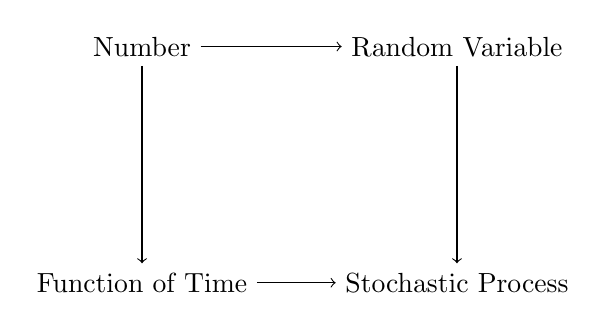
\begin{tikzpicture}
        \draw (0, 3) node[](num){Number};
        \draw (0, 0) node[](fot){Function of Time};
        \draw (4, 0) node[](sto){Stochastic Process};
        \draw (4, 3) node[](rv){Random Variable};
        \draw[->] (num) -- (rv);
        \draw[->] (num) -- (fot);
        \draw[->] (fot) -- (sto);
        \draw[->] (rv) -- (sto);
    \end{tikzpicture}
\end{center}
Therefore the two interpretations of a stochastic process are as follows:
\begin{enumerate}
    \item A sequence of random variables
    \item A random function
\end{enumerate}
Attempts to formulate the second interpretation have faced many difficulties. As such, we define a stochastic process as:
\section{DTMC}

\subsection{Review of Probability}

A \term{random variable (r.v.)}  $X$ is a real valued function of the outcomes of a random experiment.

\[ X : \Om \to R \]

Where $\Om = \bc{\w_1, \w_2, \ldots}$ is the \term{sample space} corresponding to all possible outcomes $\w_i$. The outcomes can in principle be any objects (numbers, strings, etc.). We say that $X$ maps each outcome $\w$ to a real number $\w \mapsto X\br{\w} \in \R$. \\

A \term{stochastic process} is a family of random variables $\bc{X_t}_{t \in T}$, defined on a common sample space $\Om$. $T$ is referred to as the index set for the stochastic process which is often understood as time. The index set $T$ can take a discrete spectrum,
\[ T = \bc{0, 1, 2, \ldots} \qquad \bc{X_n \mid n = 0, 1, 2, \ldots} \]
Alternatively, $T$ can take on a continuous spectrum,
\[ T = \bc{t \mid t \geq 0} = \left[ 0 , \inf \right) \]

The \term{state space} $S$ is the collection of all possible values of $X_t$'s. It is important to understand the distinction of between sample space and state space. Additionally, the state space can either have discrete or continuous spectrum. \\

A question remains, \textit{Why do we need the family of random variables to be defined on a common sample space?} The answer being that we would like to be able to discuss the joint behaviour of $X_t$'s. If $X_1$ has domain $\Om_1$ and $X_2$ has domain $\Om_2$ (where $\Om_1 \neq \Om_2$), then one can \textit{not} talk about common ideas of correlations and associations between $X_1$ and $X_2$. As such we assert that all members of a stochastic process share the same sample space domain $\Om$.

\subsection{Discrete-time Markov Chain}

A \term{discrete-time stochastic process} $\bc{X_n \mid n \in 0, 1, 2, \ldots}$ is said to be a \term{Discrete-time Markov Chain (DTMC)}  if the following conditions hold:
\begin{enumerate}
    \item The state space is at most \textit{countable}\footnote{Countable meaning there is a one-to-one mapping from the state space to the natural numbers.} (i.e. finite or countable).
    \[ S = \bc{0, 1, \ldots, k} \quad \textrm{or} \quad S = \bc{0, 1, 2, \ldots} \]
    \item \term{Markov Property}: For any $n = 0, 1, 2, \ldots$,
    \[ P\br{X_{n+1} = x_{n+1} \mid X_n = x_n, X_{n-1} = x_{n-1}, \ldots, X_{0} = x_{0}} = P\br{X_{n+1} = x_{n+1} \mid X_{n} = x_{n}} \]
\end{enumerate}
We use capital letters $X$ to denote the random variable and lower case letters $x$ to denote a specific realization or valuation of $X$. The motivation of the Markov property is that future events $X_{n+1} = x_{n+1}$ are independent of past histories $\bc{X_{i} = x_{i} \mid i = 0, 1, \ldots, n-1}$ given the immediate past state $X_{n} = x_{n}$. The intuition being that the future and the past are probabilistically independent.

\begin{center}
    \textit{Given the present, the future and the past are independent.}
\end{center}

% === Notes for GONGCHEN ===
\subsection{Transition Probability}

The \term{transition probability} from a state $i \in S$ at time $n$ to state $j \in S$ (at time $n+1$) is given by,
\[ P_{n, i, j} \defined P \br{X_{n+1}= j \mid X_{n} = i} \qquad n = 0, 1, 2, \ldots \eq \label{eq:trans_prob}\]
In full generality, the transition probability could depend on time $n$ but in this course we will restrict ourselves to transition probabilities that \textit{do not} depend on time $n$ ($P_{n, i, j} = P_{i, j}$). We say that the markov chain is \term{(time-)homogeneous} if this property holds. From now on, this will be our default setting. \\

The matrix of all transition probabilities $P = \bc{P_{i,j} \mid i,j \in S}$ is called the \term{one-step transition (probability) matrix} for $\bc{X_{n} \mid n \in T}$.
\[ P = \begin{pmatrix}
P_{00} & P_{01} & \cdots & P_{0j} & \cdots \\
P_{10} & P_{11} & \cdots & P_{1j} & \cdots \\
\vdots & \vdots & \ddots & \vdots & \cdots \\
P_{i0} & P_{i1} & \cdots & P_{ij} & \cdots \\
\vdots & \vdots & \vdots & \vdots & \ddots
\end{pmatrix} \]
The one-step transition matrix $P$ has the following properties:
\begin{enumerate}
    \item The entries of $P$ are non-negative:
    \[ P_{i,j} \geq 0 \eq \label{eq:trans_positive_entries} \]
    \item The rows of $P$ sum to unity:
    \[ \forall i : \sum_{j \in S} P_{ij} = 1 \eq \label{eq:trans_row_sum} \]
\end{enumerate}

The \term{n-step transition probability} is defined via the homogeneous property,
\[ \forall i,j \in S : P_{ij}^{(n)} \defined P\br{X_{n+m} = j \mid X_{n} = i} = P\br{X_{n} = j \mid X_{m} = i} \]
Analogously, the \term{n-step transition matrix} is the matrix,
\[ P^{(n)} = \bc{P_{ij}^{(n)} \mid i, j \in S} \]

\begin{theorem}
There is a simple relation between the n-step transition matrix $P^{(n)}$ and the one step transition matrix $P$.
\[ P^{(n)} = P^{(n-1)} \cdot P = \underbrace{P \cdot P \cdot \cdots \cdot P}_{n} = P^n \]
\end{theorem}

\begin{proof}
Proof by induction:
\[ P^{(1)} = P \note{By definition.} \]
We also have $P^{(0)} = P^{0} = \ind$ is the identity matrix. We now assume $P^{(n)} = P^{n}$. Then $\forall i,j \in S$,
\begin{align*}
    P_{ij}^{(n+1)} &= P\br{X_{n+1} = j \mid X_{0} = i} \\
    &= \sum_{k \in S} P\br{X_{n+1} = j, X_{n} = k \mid X_{0} = i} \note{Total probability}\\
    &= \sum_{k \in S} \f{P\br{X_{n+1} = j, X_{n} = k, X_{0} = i}}{P\br{X_{0} = i}} \\
    &= \sum_{k \in S} \f{P\br{X_{n+1} = j, X_{n} = k, X_{0} = i}}{P\br{X_{n} = k, X_{0} = i}}\f{P\br{X_{n} = k, X_{0} = i}}{P\br{X_{0} = i}} \\
    &= \sum_{k \in S} P\br{X_{n+1} = j \mid X_{n} = k, X_{0} = i} \cdot P\br{X_{n} = k \mid X_{0} = i} \note{Conditional total probability}\\
    &= \sum_{k \in S} P\br{X_{n+1} = j \mid X_{n} = k} \cdot P\br{X_{n} = k \mid X_{0} = i} \note{Use Markov Property}\\
    &= \sum_{k \in S} P_{kj} \cdot P_{ik}^{(n)} \note{Matrix terms}\\
    &= \br{P \cdot P^{(n)}}_{ij} \note{Matrix product}\\
    &= \br{P^{n+1}}_{ij} \note{Inductive Hypothesis}
\end{align*}
There we have proved that $P^{(n+1)} = P^{n+1}$ and so we have a completed the proof that $P^{(n)} = P^{n}$.\\
\end{proof}

This result is very fundamental. We now have a relationship between the $n$-step transition matrix and the $1$-step transition matrix (namely $P^{(n)} = P^n$). It is important to not to be confused by notation ($P^{(n)} = P^n$ is not a tautology). $P^{(n)}$ is a single matrix with entries populated by $n$-step transition probabilities while $P^n$ is a single matrix multiplied by itself $n-1$ times.

\begin{corollary}
As a corollary, we have obtained that,
\[ P^{(n)} = P^{(m)} \cdot P^{(n-m)} \quad \forall 0 \leq m \leq n \]
Or equivalently the \textbf{Chapman-Kolmogorov (C-K) Equation},
\[ P^{(n)}_{ij} = \sum_{k \in S} P^{(m)}_{ik} P^{(n-m)}_{kj} \quad \forall i,j \in S, \forall 0 \leq m \leq n \eq \label{eq:ck_equation} \]
\end{corollary}

It is very common to use the entry-wise form of the C-K equation (\cref{eq:ck_equation}) instead of the more compact but less expressive matrix form ($P^{(n)} = P^{(m)} \cdot P^{(n-m)}$). Pictorially the C-K gives reveals the following picture that holds for all Markov chains,

\begin{center}
    \begin{tikzpicture}
    \begin{scope}
        \tikzstyle{every node}=[fill=black, draw=black, circle, inner sep=1.2pt]
        \node[label=left:$i$] (i) at (0,0) {};
        \node[label=right:$j$] (j) at (4,0) {};
        \node[label=above right:$0$] (k0) at (2,2) {};
        \node[label=above right:$1$] (k1) at (2,1) {};
        \node[label=above:$k-1$] (kkm1) at (2,-1) {};
        \node[label=below right:$k$] (kk) at (2,-2) {};
    \end{scope}
    \begin{scope}[decoration={markings, mark=at position 0.5 with {\arrow{>}}}]
        \draw[postaction={decorate}] (i) -- node[above left]{$P^{(m)}_{i0}$} (k0);
        \draw[postaction={decorate}] (i) -- (k1);
        \draw[postaction={decorate}] (i) -- (kkm1);
        \draw[postaction={decorate}] (k0) -- node[above right]{$P^{(n)}_{0j}$} (j);
        \draw[postaction={decorate}] (k1) -- (j);
        \draw[postaction={decorate}] (kkm1) -- (j);

        \draw[postaction={decorate}] (i) -- node[below left]{$P^{(m)}_{ik}$}(kk);
        \draw[postaction={decorate}] (kk) -- node[below right]{$P^{(n)}_{kj}$} (j);
    \end{scope}
    \draw[dashed] (2, 2.5) -- (2, -2.5);
    \draw[dashed] (0, 2.5) -- (0, -2.5);
    \draw[dashed] (4, 2.5) -- (4, -2.5);
    \draw[] (2, 2.5) node[above]{$m$};
    \draw[] (4, 2.5) node[above]{$m+n$};
    \draw[] (0, 2.5) node[above]{$0$};
    \end{tikzpicture}
\end{center}

So far, we have only been discussing transition probabilities. We will now divert our attention to actual distributions for a stochastic process. \\

Let $\al_n = \br{\al_{n, 0}, \al_{n, 1}, \ldots}$ be the \term{probability distribution vector} for $X_n$ at time $n$.
\[ \al_{n,k} = P\br{X_n = k} \qquad \forall k \in S \]
Note that $\al_{n,k} \geq 0$ and $\sum_{k\in S} \al_{n, k} = 1$ and $n = 0, 1, 2,\ldots$. We also define the initial distribution $\al_0$,
\[ \al_0 = \br{P\br{X_0 = 0}, P\br{X_0 = 1}, \ldots} \]
\begin{theorem}
The transition probability matrix reveals the following relationship between the distribution $\al_n$ at time $n$ and the distribution $\al_0$ at time $0$,
\[ \al_n = \al_0 \cdot P^{n} \eq \label{eq:transition_dist}\]
\end{theorem}
\begin{proof}
The proof \cref{eq:transition_dist} is quite trivial:
\begin{align*}
    \forall j \in S \quad \al_{n, j} &= P\br{X_n = j} \\
     &= \sum_{i \in S} P\br{X_n = j \mid X_0 = i} \cdot P\br{X_0 = i} \\
     &= \sum_{i \in S} \al_{0, i} \cdot P_{ij}^{n} \\
     &= \al_{0, 0} \cdot P_{0j}^{n} + \al_{0, 1} \cdot P_{1j}^{n} + \ldots \\
     &= \br{\al_{0} \cdot P^{n}}_j
\end{align*}
\end{proof}
More generally, for any $n = 1, 2, \ldots$ the finite dimensional distribution can be obtained from the following process iterative process,
\begin{align*}
&\hspace{-0.5in}P\br{X_n=x_n, X_{n-1}=x_{n-1}, \ldots, X_{0}=x_{0}} = \\
&P\br{X_{0} = x_{0}} \cdot\\
&P\br{X_{1} = x_{1} \mid X_0 = x_0} \cdot\\
&P\br{\val{2} \mid \val{1}, \val{0}} \cdots \\
&P\br{\val{n} \mid \val{n-1}, \ldots, \val{0}}
\end{align*}
But by the Markov condition, it must be that,
\begin{align*}
&\hspace{-0.5in}P\br{X_n=x_n, X_{n-1}=x_{n-1}, \ldots, X_{0}=x_{0}} = \\
&P\br{X_{0} = x_{0}} \cdot\\
&P\br{X_{1} = x_{1} \mid X_0 = x_0} \cdot \\
&P\br{\val{2} \mid \val{1}} \cdots \\
&P\br{\val{n} \mid \val{n-1}}
\end{align*}
First recognize the first term on the RHS ($P\br{X_{0} = x_{0}} = \al_{0, x_0}$), and also the remaining terms are transition probabilities as per \cref{eq:trans_prob}. Therefore it must be that,
\[ P\br{X_n=x_n, X_{n-1}=x_{n-1}, \ldots, X_{0}=x_{0}} = \al_{0, x_0} P_{x_0x_1}P_{x_1x_2}\cdots P_{x_{n-1}x_n} \]
Even more generally, for $0 \leq t_1 < t_2 < \cdots < t_n$,
\[ P\br{\val{t_n}, \val{t_{n-1}}, \ldots, \val{t_{1}}} = P\br{\val{t_1}} \br{P^{t_2 - t_1}}_{x_{t_1}x_{t_2}}\br{P^{t_3 - t_2}}_{x_{t_2}x_{t_3}}\cdots\br{P^{t_{n} - t_{n-1}}}_{x_{t_{n-1}}x_{t_{n}}}  \]
Since $P\br{\val{t_1}} = \al_{t_1 x_{t_1}} = \sum_{k \in S} \al_{0, k} P^{t_1}_{k, x_{t_1}}$,
\[ \al_{t_1} = \al_{0} \cdot P^{t_1} \eq \label{eq:distribution_fundamentals} \]
\begin{remark}
\Cref{eq:transition_dist} carries a very important interpretation. The probabilistic properties of a Discrete-Time Markov Chain (DTMC) are fully characterized by two things:
\begin{enumerate}
    \item The initial distribution $\al_{0}$
    \item Transition matrix $P$
\end{enumerate}
Knowing both the initial distribution and transition matrix fully determines the distribution $\al_{n}$ for all times $n$.
\end{remark}

\subsection{Stationary Distribution (Invariant Distribution)}
In this section, we are interested in determining which distributions $\al_{0}$ remain unchanged for all time $n \in T$.
\begin{definition}
    A probability distribution $\pi = \br{\pi_0, \pi_1, \cdots}$ is called a \term{stationary (invariant) distribution} of the DTMC $\bc{X_n}_{n = 0,1, \cdots}$ with transition matrix $P$ if the following conditions hold,
    \begin{enumerate}
        \item The transition matrix does not change $\pi$:
        \[  \pi = \pi \cdot P \eq \label{eq:invariant}\]
        \item The vector $\pi$ is a valid probability distribution,
        \[ \sum_{i \in S} \pi_i = 1 \qquad \pi_i \geq 0 \eq \label{eq:prob_dist_requirements}\]
    \end{enumerate}
\end{definition}
Notice that if we posit that $\pi$ is a probability distribution, then the second condition is already satisfied. Nonetheless, in practice we are able to find candidate $\pi$'s using the the first condition and then we need to check these candidates against the second condition. In general, if $\sum_{i \in S} \pi_i$ is bounded (i.e. $\sum_{i \in S} \pi_i < \inf$) then it is possible to normalize the candidate $\pi$ in order to satisfy \cref{eq:prob_dist_requirements}. \\

\textit{Why are such $\pi$'s called stationary/invariant distributions?} Notice that \cref{eq:invariant} completely answers this question. Assume that the MC starts with initial distribution $\al_0 = \pi$ for $X_0$. In this case, the distribution of $X_1$ is determined by $P$,
\[ \al_1 = \al_0 \cdot P \]
But since $\al_0$ is $\pi$ and $\pi$ satisfies \cref{eq:invariant},
\[ \al_1 = \pi \cdot P = \pi \]
The distribution for $X_1$ is the \textit{same} as the distribution for $X_0$. This process continues,
\[ \al_2 = \al_1 \cdot P = \pi \cdot P = \pi \]
\[ \al_n = \al_0 \cdot P^n = \pi \cdot P^n = \pi \cdot P^{n-1} = \cdots = \pi \]
Thus if the Markov chain starts with a stationary/invariant distribution then its marginal distribution will \textit{never change}; hence why we refer $\pi$ as stationary. Also not that this \textit{does not} indicate that the value of $X_i$ does not change over time (it almost certainly will), but its distribution does.

\begin{example}
    Consider an electron with two states: ground $(0)$ and excited $(1)$. Let $X_n$ be the state at time $n$. At each step, with probability $\al$ the MC chains state if it is in the ground state. With probability $\be$ the MC will transition to the ground state if it is in the excited state. Then $\bc{X_n}_{n=0,1,\ldots}$ is a DTMC and its transition matrix is,
    \[ P = \kbordermatrix{
         & (0) & (1) \\
        (0) & 1 - \al & \al \\
        (1) & \be & 1 - \be \\
    } \]
    Now let us solve for the stationary distribution $\pi$.
    \[ \pi = \pi \cdot P \qquad \pi = \br{\pi_0, \pi_1} \qquad \pi_0 + \pi_1 = 1 \]
    Therefore,
    \begin{align*}
    \pi_0 &= \br{1 - \al} \pi_0 + \be \pi_1 \eq \label{eq:qe1}\\
    \pi_1 &= \al \pi_0 + \br{1 - \be} \pi_1 \eq \label{eq:qe2}
    \end{align*}
    However note that these two equations are not linearly independent. This is evident because summing \cref{eq:qe1} with \cref{eq:qe2} results in the trivial statement of $\pi_0 + \pi_1 = \pi_0 + \pi_1$. Nonetheless rearranging \cref{eq:qe1} gives,
    \[ \al \pi_0 = \be \pi_1 \implies \f{\pi_0}{\pi_1} = \f{\be}{\al} \]
    This is where we need $\pi_0 + \pi_1 = 1$.
    \[ \pi_0 = \f{\be}{\al+\be} \qquad \pi_1 = \f{\al}{\al+\be} \]
    Where $\al + \be$ is considered the normalizing constant.
\end{example}

An important remark: sometimes the candidate distribution is not normalizable. In particular, there are configurations where \cref{eq:invariant} is satisfiable but \cref{eq:prob_dist_requirements} is not. In the above example, there exists a unique stationary distribution,
\[ \pi = \br{\f{\al}{\al + \be} ,\f{\be}{\al + \be}} \]
If $\al_0 = \pi$ then we know immediately that,
\[ P\br{X_n = 0} = \f{\be}{\al+\be} \qquad P\br{X_n = 1} = \f{\al}{\al+\be} \qquad \forall n = 1, 2, \ldots\]
\begin{remark}
    By the above procedure of solving for stationary distribution is typical.
    \begin{enumerate}
        \item Use \cref{eq:invariant} to get proportions between different components of $\pi$.
        \item Use \cref{eq:prob_dist_requirements} to normalize $\pi$ and get exact values.
    \end{enumerate}
\end{remark}
\begin{remark}
    Note that if $\be = 2 \al$ then $\pi$ is always $\br{2/3, 1/3}$ regardless the actual value of $\al$.
\end{remark}
% === Notes for GONGCHEN ===
% === CONTINUE ===

\subsection{Classification of States}
\newcommand{\comm}{\leftrightarrow}
\newcommand{\acc}[2]{#1 \to #2}

Let $\bc{X_n}_{n=0,1,\ldots}$ be a DTMC with state space $S$. State $j$ is \term{accessible} from state $i$ (denoted $\acc{i}{j}$) if there exists $n = 0, 1, \ldots$ such that $P^{(n)}_{ij} > 0$. Intuitively, one can transition from state $i$ to state $j$ in finite steps $n$ with positive probability. If $i$ is also accessible from $j$, then we say $i$ and $j$ \term{communicate}, denoted as ${i}\comm{j}$.
\[ {i}\comm{j} \iff \exists m, n \geq 0, P_{ij}^{(m)} > 0, P_{ji}^{(n)} > 0 \]
The relation ``$\comm$'' either holds or does not hold for every state $i \in S$.
\begin{theorem}
The binary communication relation ``${}{\comm}$'' is in fact a equivalence relation:
\begin{itemize}
    \item Reflexivity ${i}\comm{i}$
    \item Symmetry ${i}\comm{j} \implies {j}\comm{i}$
    \item Transitivity ${i}\comm{j}, {j}\comm{k} \implies {i}\comm{k}$
\end{itemize}
\end{theorem}
\begin{proof}
First, reflexivity is easy to prove by definition. Let $n = 0$ and recognize that $P^{(0)}_{ii}$ has a certain probability by definition,
\[ P^{(0)}_{ii} = 1 \implies {i}\comm{i} \]
Second, symmetry follows by definition,
\[ P_{ij}^{(m)} > 0, P_{ji}^{(n)} > 0 \Leftrightarrow P_{ji}^{(n)} > 0, P_{ij}^{(m)} > 0 \]
Third, transitivity can be proven by letting $m$ and $n$ be the unknown quantifiers:
\[ \exists m \quad P_{ij}^{(m)} > 0, \exists n \quad P_{jk}^{(n)} > 0 \]
Then by the CK equation \cref{eq:ck_equation},
\[ P^{(m+n)}_{ik} = \sum_{l \in S} P^{(m)}_{il}P^{(n)}_{lk} \]
Let $l = j$ be a single, fixed entry in the summation,
\[ P^{(m+n)}_{ik} \geq P^{(m)}_{ij}P^{(n)}_{jk} > 0 \]
Therefore we have that $k$ is accessible from $i$ ($\acc{i}{j}$). Analogously we have that $\acc{i}{j}$ therefore ${i}\comm{k}$. \\
\end{proof}
The communication equivalence relations then divides the state space $S$ into different \term{equivalence classes}. That is, the states in one class comm with each other; the states in different classes do not comm. The equivalent classes form a \textit{partition} of the state space $S$. \\

The family $\bc{S_1, S_2, \ldots S_n}$ is a \term{partition} of $S$ if,
\begin{enumerate}
    \item $S_i \subset S \mid \forall i \in 1,2,\ldots,n$
    \item $S_i \cap S_j \neq \emptyset$ for all $i \neq j$
    \item $\bigcup_{i} S_i = S$
\end{enumerate}

We can find the equivalent classes by drawing a graph where the states in $S$ are the nodes of the graph and a directed edge is placed going from $i$ to $j$ if $j$ is accessible from $i$ in one-step: $P_{ij} > 0$. Then identifying the the equivalent classes corresponds to identifying the loops of this graph within one step. \\


\begin{example}

As an example, consider the transition matrix $P$ as follows.

\[ P = \kbordermatrix{
    & 0 & 1 & 2 & 3 & 4 \\
    0& 0.2 & 0.8 & 0 & 0 & 0 \\
    1& 0.6 & 0.4 & 0 & 0 & 0 \\
    2& 0 & 0.5 & 0 & 0.5 & 0 \\
    3& 0 & 0 & 0 & 0.7 & 0.3 \\
    4& 0 & 0 & 0 & 0.1 & 0.9} \]

The associated one-step accessibility graph is then,
\begin{center}
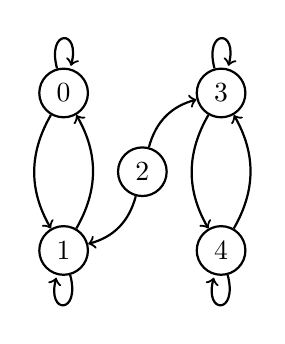
\begin{tikzpicture}
    \begin{scope}
        \tikzstyle{every node}=[fill=white, draw=black, circle, thick, text=black, scale=1.0]
        \node (0) at (0,2) {$0$};
        \node (1) at (0,0) {$1$};
        \node (2) at (1,1) {$2$};
        \node (3) at (2,2) {$3$};
        \node (4) at (2,0) {$4$};
    \end{scope}
    \begin{scope}
        \tikzstyle{every edge}=[draw, thick, ->]
        \path
        (0) edge[bend right] (1)
        (1) edge[bend right] (0)
        (0) edge[loop above] (0)
        (1) edge[loop below] (1)
        (3) edge[bend right] (4)
        (4) edge[bend right] (3)
        (3) edge[loop above] (3)
        (4) edge[loop below] (4)
        (2) edge[bend left] (3)
        (2) edge[bend left] (1);
    \end{scope}
\end{tikzpicture}
\end{center}

Where the loops of $S = \bc{0,1,2,3,4}$ form the following partition,
\[ S_1 = \bc{0,1} \quad S_2 = \bc{2} \quad S_3 = \bc{3, 4} \]
\end{example}

\begin{example}

As another example, consider the transition matrix $P$.

\[ P = \kbordermatrix{
    & 0 & 1 & 2 & 3 \\
    0& 0.5 & 0.5 & 0 & 0 \\
    1& 0.5 & 0.5 & 0 & 0 \\
    2& 0.25 & 0.25 & 0.25 & 0.25 \\
    3& 0 & 0 & 0 & 1
 } \]

The associated one-step accessibility graph is then,
\begin{center}
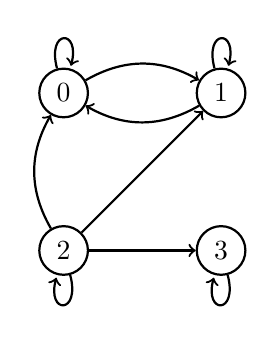
\begin{tikzpicture}
    \begin{scope}
        \tikzstyle{every node}=[fill=white, draw=black, circle, thick, text=black, scale=1.0]
        \node (0) at (0,0) {$0$};
        \node (1) at (2,0) {$1$};
        \node (2) at (0,-2) {$2$};
        \node (3) at (2,-2) {$3$};
    \end{scope}
    \begin{scope}
        \tikzstyle{every edge}=[draw, thick, ->]
        \path
        (0) edge[loop above] (0)
        (1) edge[loop above] (1)
        (2) edge[loop below] (2)
        (3) edge[loop below] (3)
        (2) edge[bend left] (0)
        (2) edge[] (3)
        (2) edge[] (1)
        (0) edge[bend left] (1)
        (1) edge[bend left] (0)
        ;
    \end{scope}
\end{tikzpicture}
\end{center}
While the loops of $S = \bc{0,1,2,3}$ form the following partition,
\[ S_1 = \bc{0,1}\quad S_2 = \bc{2} \quad S_3 = \bc{3} \]
\end{example}

\begin{example}

As another example, consider the transition matrix $P$.

\[ P = \kbordermatrix{
    & 0 & 1 & 2 & 3 \\
    0& 0.5 & 0.5 & 0 & 0 \\
    1& 0.5 & 0 & 0.5 & 0 \\
    2& 0.5 & 0 & 0 & 0.5 \\
    3& 0 & 0  & 0.5 & 0.5
 } \]

The associated one-step accessibility graph is then,
\begin{center}
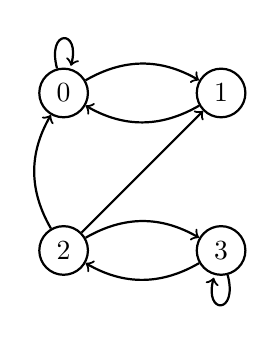
\begin{tikzpicture}
    \begin{scope}
        \tikzstyle{every node}=[fill=white, draw=black, circle, thick, text=black, scale=1.0]
        \node (0) at (0,0) {$0$};
        \node (1) at (2,0) {$1$};
        \node (2) at (0,-2) {$2$};
        \node (3) at (2,-2) {$3$};
    \end{scope}
    \begin{scope}
        \tikzstyle{every edge}=[draw, thick, ->]
        \path
        (0) edge[loop above] (0)
        (3) edge[loop below] (3)
        (2) edge[bend left] (0)
        (2) edge[bend left] (3)
        (3) edge[bend left] (2)
        (2) edge[] (1)
        (0) edge[bend left] (1)
        (1) edge[bend left] (0)
        ;
    \end{scope}
\end{tikzpicture}
\end{center}
This contrasts with the previous example because $P_{01}, P_{12}, P_{20} > 0$ implies that $0,1,2$ are in the same class and $P_{23}, P_{32} > 0$ implies that $2,3$ are in the same class. By transitivity $0,1,2,3$ are all in the same class.
\[ S_1 = \bc{0,1,2,3} \]
\end{example}

These equivalent classes are useful for Markov chains because it allows one to separate the behaviour of the equivalence classes and study them individually. A MC which has only one equivalent class is called \term{irreducible}. \\

\begin{example}
    \[ P = \kbordermatrix{
          & 0 & 1 & 2 & 3 \\
        0 & 0 & 1 & 0 & 0 \\
        1 & 0.5 & 0 & 0.5 & 0 \\
        2 & 0 & 0.5 & 0 & 0.5 \\
        3 & 0 & 0 & 1 & 0 \\
    } \]
    \begin{center}
    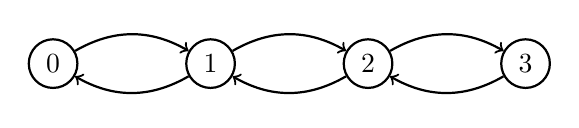
\begin{tikzpicture}
        \begin{scope}
            \tikzstyle{every node}=[fill=white, draw=black, circle, thick, text=black, scale=1.0]
            \node (0) at (0,0) {$0$};
            \node (1) at (2,0) {$1$};
            \node (2) at (4,0) {$2$};
            \node (3) at (6,0) {$3$};
        \end{scope}
        \begin{scope}
            \tikzstyle{every edge}=[draw, thick, ->]
            \path
            (0) edge[bend left] (1)
            (1) edge[bend left] (2)
            (2) edge[bend left] (3)
            (3) edge[bend left] (2)
            (2) edge[bend left] (1)
            (1) edge[bend left] (0)
            ;
        \end{scope}
    \end{tikzpicture}
    \end{center}
    Clearly if we start at state $0$, we can only go back to $0$ in $2,4,6,\ldots$ (i.e. an even number of) steps.
\end{example}
Furthermore, let us define the \term{period} of state $i$ as,

\[ d\br{i} = \gcd \bc{n \in \Z^{+} \mid P_{ii}^{n} > 0} \]

Additionally, if $P_{ii}^{n} = 0$ holds for all $n > 0$, we say that $d\br{i} = \inf$. If the period of $i$ happens to be $d\br{i} = 1$ then the state $i$ is said to be \term{aperiodic}. Alternatively, locus of steps that we can go back by are \textit{co-prime}. A MC is called aperiodic if all its states $S$ are aperiodic.\\

Note that $P_{ii} < 0$ then the greatest common divisor must be one. This implies that $d_i = 1$. In this case, the state is immediately aperiodic.\\

The period of a state is useful do to the following theorem,

\begin{theorem}
\label{thm:period_class_prop}
The period of a state is a class property. If ${i}\comm{j}$, then $d\br{i} = d\br{j}$.
\end{theorem}

\begin{proof}
If $i = j$ we are already done. If $i \neq j$, since ${i}\comm{j}$, then $\exists n, m$ such that,
\[ P_{ij}^{n} > 0 \quad P_{ji}^{m} > 0 \]
Then for any $l$ such that $P^{l}_{jj} > 0$,
\[ P_{ii}^{n+m+l} \geq P_{ij}^{n}P_{jj}^{l}P_{ji}^{m} \eq \label{eq:period_class_prop_2} \]
Because $P_{ij}^{n}P_{jj}^{l}P_{ji}^{m}$ happens to be a specific way for $P_{ii}^{n+m+l}$ to occur. Since ${i}\comm{j}$ and $l$ was chosen carefully,
\[ P_{ii}^{n+m+l} > 0 \]
Moreover, we also have that,
\[ P_{ii}^{n+m} \geq P_{ij}^{n}P_{ji}^{m} \eq \label{eq:period_class_prop_1}\]
Since $d\br{i}$ divides both $n+m$ and $n+m+l$ by \cref{eq:period_class_prop_1,eq:period_class_prop_2}, then $d\br{i}$ also divides $l$. This holds for all $l$ such that $P_{ii}^{l}>0$. This implies that $d\br{i}$ is a common divisor of $\bc{l \mid P_{jj}^{l} > 0}$ an thus $d\br{i}$ divides,
\[ d\br{j} = \gcd \bc{l \mid P_{jj}^{l} > 0} \]
By symmetry $d\br{j}$ divides $d\br{i}$. Therefore $d\br{i} = d\br{j}$. \\
\end{proof}

\begin{remark}
It is important to note that $d\br{i} = k \not\Rightarrow P_{ii}^{(k)} > 0$. As a counterexample consider the following one step accessibility graph,
\begin{center}
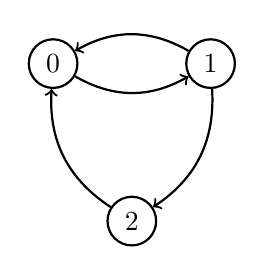
\begin{tikzpicture}
    \begin{scope}
        \tikzstyle{every node}=[fill=white, draw=black, circle, thick, text=black, scale=1.0]
        \node (0) at (-1,2) {$0$};
        \node (1) at (1,2) {$1$};
        \node (2) at (0,0) {$2$};
    \end{scope}
    \begin{scope}
        \tikzstyle{every edge}=[draw, thick, ->]
        \path
        (0) edge[bend right] (1)
        (1) edge[bend right] (0)
        (2) edge[bend left] (0)
        (1) edge[bend left] (2);
    \end{scope}
\end{tikzpicture}
\end{center}
Evidently,
\[ P^{(2)}_{00} > 0 \quad P^{(3)}_{00} > 0 \]
So we have $d\br{0} = 1$ because $d\br{0} = \gcd\bc{2,3,\ldots}$. However this doesn't imply that $P_{00}^{(1)} > 0$ because we do have that $P^{(1)}_{00} = 0$
\end{remark}

\begin{remark}
If the MC is irreducible (having only one class) then all the states have the same period. In this case we ascribe the entire MC the period $d\br{i}$ for some representative $ i \in S$.
\end{remark}

\begin{remark}
    If the period of $i$ is $d_i = 1$ then there exists some $N$ such that $P_{ii}^{(n)} > 0$ for any $n \geq N$. Intuitively, if state $i$ is aperiodic then after a long time, the probability of going back to $i$ is always positive.
\end{remark}

\subsection{Recurrence and Transience}
In order to define transience and recurrence, let $T_i$ be the waiting time of a MC to visit/revisit state $i$ for the first time since time $0$.
\[ T_i = \min \bc{n > 0 : X_n = i} \]
Of course we have that $\bc{n > 0 : X_n = i}$ is a random collection of numbers and also $\min\bc{n > 0 : X_n = i}$ is a random number. Therefore $T_i$ is a random variable. Notice that if $T_i = \inf$ if the MC never returns to state $i$.
\begin{definition}
    A state $i$ is called \term{transient} if,
    \[ P\br{T_i < \inf \mid X_0 = i} < 1 \]
    Or equivalently,
    \[ P\br{T_i = \inf \mid X_0 = i} > 0 \]
    We say that the MC never goes back to state $i$ with positive probability.
\end{definition}
Moreover,
\begin{definition}
    A state $i$ is \term{recurrent} if,
    \[ P\br{T_i < \inf \mid X_0 = i} = 1 \]
    Or equivalently,
    \[ P\br{T_i = \inf \mid X_0 = i} = 0 \]
    We say that the MC always goes back to $i$.
\end{definition}
\begin{remark}
    If we have that $P\br{T < \inf} = 1$ then it does not imply that $\Exp\br{T} < \inf$. As a counter example, let $s_p = 2^{p}$ for $p = 1, \ldots, \inf$,
    \[ P\br{T = s_p} = \f{1}{s_p} \]
    Where the expectation of $T$ is unbounded,
    \[ \Exp\br{T} = \sum_{p=1}^{\inf} s_p \f{1}{s_p} = \sum_{p=1}^{\inf} 1 = \inf \]
\end{remark}
To make the distinction,
\begin{definition}
    A recurrent state $i$ is said to be \term{positive recurrent} if,
    \[ \Exp\br{T_i \mid X_0 = i} < \inf \]
    A recurrent state $i$ is said to be \term{null recurrent} if,
    \[ \Exp\br{T_i \mid X_0 = i} = \inf \]
\end{definition}

\begin{example}
    Consider the following example with transition matrix,
    \[ P \kbordermatrix{
          & 0 & 1 & 2 \\
        0 & \f12 & \f12 & 0 \\
        1 & 0 & \f12 & \f12 \\
        2 & 0 & 0 & 1 \\
    } \]
    And MC graphically expressed as,
    \begin{center}
    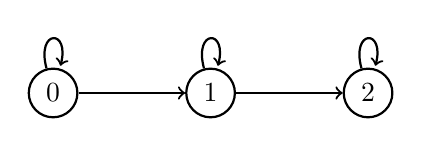
\begin{tikzpicture}
        \begin{scope}
            \tikzstyle{every node}=[fill=white, draw=black, circle, thick, text=black, scale=1.0]
            \node (0) at (0,0) {$0$};
            \node (1) at (2,0) {$1$};
            \node (2) at (4,0) {$2$};
        \end{scope}
        \begin{scope}
            \tikzstyle{every edge}=[draw, thick, ->]
            \path
            (0) edge[] (1)
            (1) edge[] (2)
            (0) edge[loop above] (0)
            (1) edge[loop above] (1)
            (2) edge[loop above] (2);
        \end{scope}
    \end{tikzpicture}
    \end{center}
    Given that $X_0 = 0$ there are only two possibilities for transitions,
    \[ P\br{\underbrace{X_1 = 0 \mid X_0 = 0}_{T_0 = 1}} = P\br{\underbrace{X_1 = 1 \mid X_0 = 0}_{T_0 = \inf}} = \f12 \]
    The second term is recognized as $T_0 = \inf$ because after transitioning to state $1$, it is impossible to return to state $0$. This tells us that,
    \[ P\br{T_0 < \inf \mid X_0 = 0} = \f{1}{2} < 1 \]
    Therefore state $0$ is said to be transient. Analogously we have that state $1$ is also transient. Given $X_0 = 2$, $P\br{\underbrace{X_1 = 2 \mid X_0 = 2}_{T_2=1}} = 1$ we have that,
    \[ P\br{T_2 < \inf \mid X_0 = 2} - 1 \]
    Which tells is that state $2$ is recurrent.
\end{example}
In general, the distribution of $T_i$ is very hard to derive. In particular it will be hard to know whether $T_i$ takes value $\inf$ and with what probability. This suggests that we will need handier criteria for recurrence/transience. \\

To facilitate this define $f_{ii} = P\br{T_i < \inf \mid X_0 = i}$ and,
\[ f_{ij} = P\br{T_j < \inf \mid X_0 = i} \]
We also defined $V_i$ to be the number of times that the MC visits state $i$,
\[ V_i = \sum_{n=1}^{\inf} \ident_{\bc{X_n = i}} \]
First consider the case that $i$ is transient. If $i$ is transient, then it must be that $f_{ii} < 1$. This can be seen from the definition of $T_i$. The PMF is,
\[ P\br{V_i = k \mid X_0 = i} = f_{ii}^{k} \br{1 - f_{ii}} \]
This can be derived by considering that if the MC is to visit state $i$ exactly $k$ times but not more than $k$ times.
\[ P\br{V_i = k \mid X_0 = i} = \bs{P\br{T_i < \inf \mid X_0 = i}}^{k} \bs{P\br{T_i = \inf \mid X_0 = i}} \]
This PMF tells us that $V_i + 1$ follows a geometric distribution with parameter $1 - f_{ii}$,
\[ V_i + 1 \sim \Geo\br{1 - f_{ii}} \]
In particular, $P\br{V_i < \inf \mid X_0 = i} = 1$. Therefore if $i$ is transient, it is visited only finitely many times with probability $1$. Afterwards, the MC will leave state $i$ forever sooner or later.\\

Second consider the case that $i$ is recurrent. If state $i$ is recurrent, then $f_{ii} = 1$ by definition. The we have that,
\[P\br{V_i = k\mid X_0 = i} = 0 \quad \forall k = 0, 1, \ldots  \]
Since $V_i$ can not take on any finite values, it must be that
\[ P\br{V_i = \inf\mid X_0 = i} = 1 \]
If the MC starts from recurrent state $i$ is will visit that state infinitely many times. Before identifying our more versatile criteria, we generalize some of these notions.
\subsection{Recurrence and Transience Again}
For $n \in \Z^{+}$ define,
\[ f_{ij}^{(n)} = P \br{X_n = j, X_{n-1} \neq j, \cdots, X_{1} \neq j \mid X_0 = i} \quad \forall i,j \in S \]
Intuitively, $f_{ij}^{(n)}$ is the probability that $X$ visits state $j$ at time $n$ for the first time since $X_0 = i$. A looming question: What is the relation between $f_{ij}^{(n)}$ and $P_{ij}^{(n)}$? First notice that,
\[ P_{ij}^{(n)} \geq f_{ij}^{(n)} \]
These reads: the probability that $X$ visits $j$ at time $n$ is more larger that the probability that $X$ visits $j$ at time $n$ provided it did not visit $j$ prior. A more detailed equality is the following,
\[ P_{ij}^{(n)} = \sum_{k = 1}^{n} f_{ij}^{(k)}P_{jj}^{(n-k)} \eq \label{eq:recurrence_form}\]
Expanded out gives,
\[ P_{ij}^{(n)} = f_{ij}^{(n)} + \sum_{k = 1}^{n-1} f_{ij}^{(k)}P_{jj}^{(n-k)} \]
\begin{proof}
\begin{align*}
P_{ij}^{(n)} & = P\br{X_n = j \mid X_0 = i} \\
& = \sum_{k=1}^{n} P\br{X_n = j, \text{$X$ first visits $j$ at time $k$} \mid X_0 = i} \\
& = \sum_{k=1}^{n} P\br{X_n = j, \mid \text{$X$ first visits $j$ at time $k$}, X_0 = i} \cdot P\br{\text{$X$ first visits $j$ at time $k$} \mid X_0 = i} \\
& = \sum_{k=1}^{n} P\br{X_n = j, \mid X_k = j, X_{k-1} \neq j, \ldots, X_{1} \neq j, X_0 = i} \cdot P\br{X_k = j, X_{k-1} \neq j, \ldots, X_{1} \neq j \mid X_0 = i} \\
& = \sum_{k=1}^{n} P\br{X_n = j, \mid X_k = j, X_{k-1} \neq j, \ldots, X_{1} \neq j, X_0 = i} \cdot f_{ij}^{(k)} \\
& = \sum_{k=1}^{n} P\br{X_n = j, \mid X_k = j} \cdot f_{ij}^{(k)} \note{Markov Condition} \\
& = \sum_{k=1}^{n} P^{(n-k)}_{jj} \cdot f_{ij}^{(k)}
\end{align*}
\end{proof}
In fact \cref{eq:recurrence_form} defines a recurrence relation to compute $f_{ij}^{(n)}$ from $f_{ij}^{(k)}$ where $k < n$,
\[ f_{ij}^{(n)} = P_{ij}^{(n)} - \sum_{k=1}^{n-1} f_{ij}^{(k)} P_{jj}^{(n+k)} \]
We now define $f_{ij}$ \textit{without} the superscript to be,
\[ f_{ij} = \sum_{n=1}^{\inf} f_{ij}^{(n)} \]
The probability that $X$ will \textit{ever} reach state $j \in S$ provided it started at $i$ ($f_{ij} \leq 1$). Whether or not $f_{ij}$ is certain or not defines the following two properties.\\

A state $i$ is called \term{transient} if $f_{ii} < 1$; and \term{recurrent} if $f_{ii} = 1$. Intuitively, $f_{ii}$ is the probability the MC returns to state $i$ given it started in state $i$. If $i$ is transient, then there is a non-negative probability that the MC does not return to $i$ and if $f_{ii} = 1$ then the MC always returns to state $i$.\\

Another way to characterize recurrence and transience: Define $V_i$ to be the total number of times the MC (re)visits $i$ after time $0$. In more mathematical terms,
\[ V_i = \sum_{n=1}^{\inf} \ind_{\bs{X_n = i}} \]
Where $\ind_{\bs{X_n = i}}$ is the indicator defined by,
\[ \ind_{\bs{X_n = i}} = \begin{cases}
    1 & X_n = i \\
    0 & X_n \neq i
\end{cases} \]
If $f_{ii} < 1$ we have that the probability of visiting state $i$ $k$ times is given by,
\begin{align*}
    P\br{V_i = k \mid X_0 = i} &= \underbrace{f_{ii} \cdot f_{ii} \cdots f_{ii}}_{k}\underbrace{\br{1 - f_{ii}}}_{\text{never return}}
\end{align*}
Where $\br{1 - f_{ii}}$ is necessary because it guarantees that we never return to state $i$ more that $k$ times. Given $X_0 = i$, $V_i$ follows a geometric distribution with parameter $\br{1 - f_{ii}}$. Thus,
\[ \Exp\br{V_i \mid X_0 = i} = \f{f_{ii}}{1 - f_{ii}} < \inf \]
Therefore if $i$ is transient, there a finite number revisits are expected. In contrast if $f_{ii} = 1$ we have that,
\[ \Exp\br{V_i \mid X_0 = i} = \lim_{f_{ii} \to 1}\f{f_{ii}}{1 - f_{ii}} \to \inf \]
Recalling our construction of the random variable $V_i$ we can alternatively write $\Exp\br{V_i \mid X_0 = i}$ as,
\begin{align*}
    \Exp\br{V_i \mid X_0 = i}
    &= \Exp\br{\sum_{n=1}^{\inf} \ident_{\bc{X_n = i}} \mid X_0 = i}  \\
    &= \sum_{n=1}^{\inf}\Exp\br{ \ident_{\bc{X_n = i}} \mid X_0 = i}  \\
    &= \sum_{n=1}^{\inf}P\br{X_n = i \mid X_0 = i}  \\
    &= \sum_{n=1}^{\inf}P_{ii}^{(n)}  \\
    &= \sum_{n=1}^{\inf}P_{ii}^{n}
\end{align*}
Therefore we have equivalent criteria for recurrent and transience for a state $i$.
\begin{center}
    \begin{tabular}{|c|c|}
        \hline
        recurrent & transient \\
        \hline
        $P\br{T_i < \inf \mid X_0 = i} = 1$ & $P\br{T_i < \inf \mid X_0 = i} < 1$ \\
        $P\br{V_i = \inf \mid X_0 = i} = 1$ & $P\br{V_i < \inf \mid X_0 = i} = 1$ \\
        $\Exp\br{V_i \mid X_0 = i} = \inf$ & $\Exp\br{V_i \mid X_0 = i} < \inf$ \\
        $\sum_{n=1}^{\inf}P_{ii}^{n} = \inf$ & $\sum_{n=1}^{\inf}P_{ii}^{n} < \inf$ \\
        \hline
    \end{tabular}
\end{center}
The final criteria being the easiest to use. \\

A final criteria we can consider is,
\[ \Exp\br{V_i \mid X_0 = i} = \sum_{k=1}^{\inf} P\br{V_i \geq k \mid X_0 = i} \eq \label{eq:Mgeqk}\]
The proof of \cref{eq:Mgeqk} is left as an exercise to the reader. Clearly if $f_{ii} = 1$,
\[ P\br{V_i \geq k \mid X_0 = i} = {f_{ii}}^k = 1 \quad \forall k \eq \label{eq:mmmm}\]
Therefore,
\[ \Exp\br{V_i \mid X_0 = i} = \sum_{k=1}^{\inf} 1 = \inf\]
\begin{theorem}
Therefore $i$ is recurrent if and only if $P\br{V_i \geq k \mid X_0 = i} = \inf$ and $i$ is transient if and only if only if $P\br{V_i \geq k \mid X_0 = i} < \inf$.
\end{theorem}
\begin{remark}
We actually also have that $i$ is recurrent if and only if $V_i = \inf$. This can be seen from \cref{eq:mmmm}. Since $P\br{V_i \geq k \mid X_0 = i}$ is strictly positive for all $k$, then $V_i = \inf$. Analogously, we have that $i$ is transient if and only if $V_i < \inf$.
\end{remark}
Yet \textit{another} way to characterize recurrence and transience is much more tractable. First,
\begin{theorem}
    The expectation of the indicator is given by $\Exp\br{\ind_{A}} = P\br{A}$ for any event $A$.
\end{theorem}
Therefore,
\begin{align*}
\Exp\br{V_i \mid X_0 = i} &= \Exp\br{\sum_{n=1}^{\inf} \ind_{\bs{X_n = i}} \mid X_0 = i} \\
&= \sum_{n=1}^{\inf}\Exp\br{ \ind_{\bs{X_n = i}} \mid X_0 = i} \note{Fubini's Theorem} \\
&= \sum_{n=1}^{\inf}P\br{ X_n = i \mid X_0 = i}\\
&= \sum_{n=1}^{\inf}P_{ii}^{(n)}
\end{align*}
Thus $i$ is recurrent if and only if $\sum_{n=1}^{\inf}P_{ii}^{(n)} = \inf$ and $i$ is transient if and only if $\sum_{n=1}^{\inf}P_{ii}^{(n)} < \inf$.\\

\begin{theorem}
Recurrence/transience are class properties. If $i \comm j$ and $i$ is recurrent (transient), then $j$ is recurrent (transient).
\end{theorem}
\begin{proof}
    Since $i \comm j$, there must be times $\exists m,n \geq 0$ that permit $i$ to access $j$ and $j$ to access $i$,
    \[ P_{ij}^{(m)} > 0 \qquad P_{ji}^{(n)} > 0 \]
    Suppose that $i$ is recurrent, then $\sum_{l=1}^{\inf}P_{ii}^{(l)} = \inf$. We now what to show that $\sum_{s=1}^{\inf}P_{jj}^{(s)}$ is infinite as well. Since $m,n \geq 0$ we can drop positive terms to get,
    \[ \sum_{s=1}^{\inf}P_{jj}^{(s)} \geq \sum_{s=n+m+1}^{\inf}P_{jj}^{(s)} \]
    Now exchange the variables of summation by letting $l = s- n-m$,
    \[ \sum_{s=1}^{\inf}P_{jj}^{(s)} \geq \sum_{l=1}^{\inf}P_{jj}^{(n+l+m)} \]
    Then by the C-K equation (\cref{eq:ck_equation}) a example path from $j$ to $j$ is to transition $j \to i \to i \to j$ in steps $m, l, n$ respectively,
    \[ \sum_{l=1}^{\inf}P_{jj}^{(n+l+m)} \geq  \sum_{l=1}^{\inf}P_{ji}^{(n)}P_{ii}^{(l)}P_{ij}^{(m)} = P_{ji}^{(n)}P_{ij}^{(m)}\bc{\sum_{l=1}^{\inf}P_{ii}^{(l)}} \]
    But since $i$ is recurrent, $\sum_{l=1}^{\inf}P_{ii}^{(l)} = \inf$. Also, $P_{ji}^{(n)}P_{ij}^{(m)} > 0$ by the choice of $m,n$. Therefore $\sum_{l=1}^{\inf}P_{jj}^{(n+l+m)} = \inf$ and thus $\sum_{s=1}^{\inf}P_{jj}^{(s)} = \inf$. Therefore $j$ is also recurrent.
\end{proof}
\begin{corollary}
    If $i \comm j$ and $i$ is transient, then $j$ is transient.
\end{corollary}
As a result, if we know that if a MC is irreducible (admitting only one class), then either all states are transient or they are all recurrent. In such cases we can say that the MC itself is recurrent/transient.

\begin{theorem}
    If an irreducible MC has a finite state space, then it is recurrent.
\end{theorem}

To see why this is true, if all states are transient then each state $i \in S$ has a time $k$ that is the \textit{last} visit time for all states, this is impossible because $P_{ij} \neq 0$ for at least some choice $i,j \in S$.

\begin{remark}
    We can actually show that the MC must be positive recurrent if the state space is finite and the MC is irreducible.
\end{remark}

\begin{theorem}
    If $i$ is recurrent, and $i$ does not communicate with $j$, then $P_{ij} = 0$.
\end{theorem}
\begin{proof}
    Proof by contradiction. Assume that $P_{ij} > 0$. Since $i$ and $j$ do not communicate, then either $j$ is not accessible from $i$ or vice versa. But if $P_{ij}>0$ then $j$ is accessible from $i$. It must be that $i$ is not accessible from $j$. Recall that $f_{ii}$ is the probability that the MC ever revisits the state $i$ given the starting state was $i$. Therefore $1 - f_{ii}$ is the probability that the MC never revisits state $i$.
    \[ f_{ii} \leq 1 - P_{ij} < 1 \]
    This inequality holds because if $X_1 = j$ then the MC never revisits $i$ ($i$ is not accessible from $j$). But there are other ways it never revisits $i$. Therefore,
    \[ P\br{X_1 = j \mid X_0 = i} = P_{ij} \leq P\br{\text{MC never revisits $i$} \mid X_0 = i} \]
    But if $f_{ii} < 1$, then $i$ is not recurrent; it is transient. Therefore the assumption that $P_{ij} > 0$ is wrong; $P_{ij} = 0$.
\end{proof}

\subsection{Limiting Distribution}

In this section we are interested in the \term{limiting transition probability} and the \term{limiting distribution} of a MC.
\[ \lim_{n \to \inf} P^{(n)}_{ij} \qquad \lim_{n \to \inf} P\br{X_n = j} \]
To keep things simple, we assume that the process $\bc{X_n}_{n=0,1,2,\dots}$ is irreducible.

\begin{theorem}
    \term{Basic Limit Theorem:} Let $\bc{X_n}_{n=0,1,\ldots}$ be an irreducible, aperiodic and positive recurrent DTMC, then a stationary distribution $\pi = \br{\pi_0, \pi_1, \ldots}$ exists. Moreover we have,
    \[ \lim_{n \to \inf} P^{(n)}_{ij} = \lim_{n \to \inf} \f{\sum_{k=1}^{n} \ident_{\bc{X_k = j}}}{n} = \f{1}{\Exp\br{T_j \mid X_0 = j}} = \pi_j \qquad \forall i,j \in S \]
    Where $T_j = \min\bc{n > 0, X_n = j}$. In words, the limiting distribution is equal to the long-run fraction of time spent in $j$ is equal to the stationary distribution. Note that this does not depend on the starting state $i$.
\end{theorem}

\todo[TC]{Missed a lecture}
By examining foil theorems, we have seen that irreducibility is related to the uniqueness of the stationary distribution, aperiodicity is related to the existence of $\lim_{n \to \inf} P^{(n)}_{ij}$ and positive recurrence is related to the existence of stationary distribution. \\

\begin{example}
    Let us have an electron with two states and $P$ given by,
    \[ P = \begin{pmatrix}
        1 - \al & \al \\
       \be & 1 - \be \\
    \end{pmatrix} \]
    Where $\lim_{n \to \inf} P^n$ becomes,
    \[ \lim_{n \to \inf} P^n = \begin{pmatrix}
        \f{\al}{\al + \be} & \f{\be}{\al + \be} \\
        \f{\al}{\al + \be} & \f{\be}{\al + \be} \\
    \end{pmatrix} \]
    It is important to notice that $\lim_{n \to \inf} P^n$ does not depend on the row considered (i.e. the initial state $i$ considered). We have the stationary distribution is,
    \[ \pi = \begin{pmatrix}
        \f{\al}{\al + \be} & \f{\be}{\al + \be} \\
    \end{pmatrix} \]
    So we verify that $\pi_j = \lim_{n \to \inf} P_{ij}^{(n)}$. Also given that we start from state $X_0 = 0$, then clearly,
    \begin{align*}
        P\br{T_0 = 1 \mid X_0 = 0} &= 1 - \al \\
        P\br{T_0 = 2 \mid X_0 = 0} &= \al \be \\
        P\br{T_0 = 3 \mid X_0 = 0} &= \al \br{1 - \be} \be \\
        P\br{T_0 = k \mid X_0 = 0} &= \al  \br{1 - \be}^{k-2}  \be   \quad \forall k= 2, 3, \ldots
    \end{align*}
    Where $\al$ represents leaving state $0$ and $\be$ represents returning to state $0$ at step $k$. $\br{1- \be}^{k-2}$ represents not returning to $0$ until step $k$. We then obtain the expectation,
    \[ \Exp\br{T_0 \mid X_0 = 0} = 1 - \al + \sum_{k=2}^{\inf} \al \br{1- \be}^{k-2} \be k \]
    We then split this sum into two components,
    \[ \Exp\br{T_0 \mid X_0 = 0} = 1 - \al + \sum_{k=2}^{\inf} \al \br{1- \be}^{k-2} \be \br{k - 1} + \sum_{k=2}^{\inf} \al \br{1- \be}^{k-2} \be\]
    We then notice that $\br{1- \be}^{k-2} \be$ is the pmf of $\Geo\br{\be}$ while the first sum ($\sum_{k=2}^{\inf} \br{1- \be}^{k-2} \be \br{k - 1}$) is simply the expectation of $\Geo\br{\be}$. Therefore,
    \[ \Exp\br{T_0 \mid X_0 = 0} = 1 - \al + \al \f{1}{\be} + \al = 1 + \f{\al}{\be} = \f{\al + \be}{\be}\]
    We verify that $\Exp\br{T_0 \mid X_0 = 0} = \f{1}{\pi_0}$. Of course, this is one of the few cases where we can explicitly verify the predictions of the Basic Limit Theorem. In the future, we will accept the BLT and move forward.
    \end{example}

    \subsection{Generating Function}
    Before defining the generating function we recall the moment generating function $\Mom_k\br{t} = \Exp\br{e^{t X}}$. The moment generating function is defined for any distribution $X$. However the generating function is defined for distributions over the non-negative integers.
    \begin{definition}
        Let $p = \br{p_0, p_1, \ldots}$ be a distribution over the non-negative integers $\bc{0,1,2,\ldots}$ such that $p_i \geq 0$ and $\sum_{i} p_i = 1$. Let $\xi$ be a random variable following distribution $p : \xi \sim p$. Then the generating function of $\xi$ (or for $p$) is defined as,
        \[ \varphi\br{s} = \Exp\br{s^{\xi}} = \sum_{k = 0}^{\inf} s^k p_k \quad \forall 0 \leq s \leq 1\]
    \end{definition}
    The generating function is useful for the following properties.
    \begin{enumerate}
        \item The generating function always intersects two points: $\varphi\br{0} = p_0$, $\varphi\br{1} = 1$
        \item The generating function determines the distribution:
        \[ p_k = \f{1}{k!} \f{\dif^k \varphi \br{s}}{\dif s^k} \bigg|_{s=0} \]
        \begin{proof}
            In order to proof the second property, simply take $\varphi\br{s}$ as a sum,
            \[ \varphi\br{s} = p_0 + p_1 s^1 + \cdots + p_{k-1} s^{k-1}+ p_{k} s^{k}+ p_{k+1} s^{k+1} + \cdots \]
            Then the $k$-th derivative of $\varphi\br{s}$ is,
            \[ \f{\dif^k \varphi \br{s}}{\dif s^k} = k ! p_{k} s^{0} + \f{\br{k+1}!}{1!} p_{k+1} s^{1} + \f{\br{k+2}!}{2!} p_{k+2} s^{2} + \cdots \eq \label{eq:generating_sum}\]
            But when evaluated at $s = 0$,
            \[ \f{\dif^k \varphi \br{s}}{\dif s^k} \bigg|_{s=0} = k! p_k \]
        \end{proof}
        \begin{remark}
            In particular, if we restrict ourselves to $s \geq 0$ \cref{eq:generating_sum} determines,
            \begin{align*}
            \varphi'\br{s} \geq 0 &\implies \varphi\br{s} \text{ is increasing} \\
            \varphi''\br{s} \geq 0 &\implies \varphi\br{s} \text{ is convex} \\
            \end{align*}
        \end{remark}
        \item Let $\xi_1, \xi_2, \ldots, \xi_n$ be independent random variables with generating functions $\varphi_1, \ldots, \varphi_2$. Then if $X = \xi_1 + \cdots + \xi_n$ then,
        \[ \varphi_X\br{s} = \varphi_1 \br{s} \cdots \varphi_n \br{s} \]
        \begin{proof}
            The proof of which is similar to the analogous property for moment generating functions.
            \begin{align*}
                \varphi_X\br{s}
                &= \Exp\br{s^{X}}\\
                &= \Exp\br{s^{\xi_1 + \cdots + \xi_n}}\\
                &= \Exp\br{s^{\xi_1}\cdots s^{\xi_n}}\\
                &= \Exp\br{s^{\xi_1}}\cdots \Exp\br{s^{\xi_n}} \note{Independence}\\
                &= \varphi_1\br{s}\cdots\varphi_n\br{s}
            \end{align*}
        \end{proof}
        \item If we take the derivative evaluated at the point $s = 1$ then,
        \[ \f{\dif^k \varphi\br{s}}{\dif s^k} \bigg|_{s=1} = \f{\dif^k \Exp\br{s^{\xi}}}{\dif s^k} \bigg|_{s=1} = \Exp\br{ \f{\dif^k s^{\xi}}{\dif s^k}} \bigg|_{s=1} = \Exp\br{\xi\br{\xi-1}\cdots\br{\xi - k + 1}s^{\xi - k}}\bigg|_{s=1} = \Exp\br{\f{\xi!}{k!}} \]
        Clearly this is not the moment generating function but it is intimately related. In particular $\Exp\br{\xi} = \varphi\br{1}$ and,
        \begin{align*}
        \Var\br{\xi}
        &= \Exp\br{\xi^2} - \br{\Exp\br{\xi}}^2 \\
        &= \Exp\br{\xi\br{\xi - 1}} + \Exp\br{\xi} - \br{\Exp\br{\xi}}^2 \\
        &= \varphi'\br{1} + \varphi'\br{1} - \br{\varphi'\br{1}}^2
        \end{align*}
    \end{enumerate}
    A characteristic plot is depicted below.
    \begin{center}
        \begin{tikzpicture}
            \draw[<->] (3, 0) node[right]{$s$} -- (0,0) -- (0, 3) node[above]{$\varphi\br{s}$};
            \draw [red] plot [smooth, tension=0.7] coordinates { (0,0.5) (1+0.4,1-0.2) (2.5, 2.5)};
            \draw[dashed] (2.5, 0) node[below]{$1$} -- (2.5,2.5) -- (0, 2.5) node[left]{$1$};
            \draw (0, 0.5) node[left]{$p_0$};
        \end{tikzpicture}
    \end{center}

    \subsection{Branching Processes}
    Consider a population of organism such that each organism, at the end of its lifetime, produces a random number of $\xi$ offsprings with probability $P\br{\xi = k} = p_k$ for $k = 0, 1, 2, \ldots$ such that $p_k \geq 0$ and $\sum_k p_k = 1$. The number of offsprings between different individuals are independent. We consider the first set of organisms the \term{ancestor generation} and each subsequent generation, \term{generation $1,2,3,\ldots$}. \\

    We let $X_n$ be the number of individuals or the population in the $n$-th generation. We restrict or focus to $X_0 = 1$. Then $X_{n+1}$ is,
    \[ X_{n+1} = \xi^{(n)}_1 + \cdots + \xi^{(n)}_{X_n} \]
    Where $\xi^{(n)}_1, \ldots, \xi^{(n)}_{X_n}$ are the independent copies of $\xi$ and $\xi_{i}^{(n)}$ is the number of offsprings of the $i$-th individual in generation $n$. \\

    What is the mean and variance of $X_n$? First assume that $\Exp\br{\xi} = \mu$ and $\Var\br{\xi} = \si^2$. Remember that $\xi$ is the number of offspring produced by an individual of the population. To find $\Exp\br{E_n}$ first make use of the $\Exp\br{X_{n+1}}$.
    \begin{align*}
    \Exp\br{X_{n+1}}
    &= \Exp\br{\xi^{(n)}_1 + \cdots + \xi^{(n)}_{X_n}}\\
    &= \Exp\br{\Exp\br{\xi^{(n)}_1 + \cdots + \xi^{(n)}_{X_n}\mid X_n}}\\
    &= \Exp\br{\mu X_n}\\
    &= \mu \Exp\br{X_n}
    \end{align*}
    Recursively if $\Exp\br{X_{n+1}} = \mu \Exp\br{X_n}$, then we have that,
    \[ \Exp\br{X_n} = \mu^n \Exp\br{X_0} = \mu^n  \quad \forall n = 0, 1, 2, \ldots \]
    Next we find $\Var\br{X_{n+1}}$ using,
    \[ \Var\br{X_{n+1}} = \Exp\br{\Var\br{X_{n+1} \mid X_n}} + \Var\br{\Exp\br{X_{n+1} \mid X_n}} \]
    Examine the first term and make use of Wald's identity,
    \begin{align*}
        \Exp\br{\Var\br{X_{n+1} \mid X_n}}
        &= \Exp\br{\Var\br{\xi^{(n)}_1 + \cdots + \xi^{(n)}_{X_n} \mid X_n}} \\
        &= \Exp\br{\si^2 X_n} \\
        &= \si^2 \mu
    \end{align*}
    \[ \Var\br{\Exp\br{X_{n+1} \mid X_n}} = \Var\br{\mu X_n} = \mu \Var\br{X_n} \]
    Combining these results and we arrive at the recursive relation,
    \[ \Var\br{X_{n+1}} = \si^2 \mu^n + \mu^2 \Var\br{X_n} \]
    With initial variance $\Var\br{X_1} = \si^2$. Therefore,
    \[ \Var\br{X_2} = \si^2 \mu^1 + \mu^2 \si^2 = \si^2 \br{\mu^1 + \mu^2} \]
    Similarly for $n = 3$,
    \[ \Var\br{X_3} = \mu^2 \si^2  + \mu^2 \Var\br{X_2} = \si^2 \br{\mu^2 + \mu^3 + \mu^4} \]
    Altogether,
    \[ \Var\br{X_n} = \si^2 \br{\mu^{n-1} + \cdots + \mu^{2n-2}} \]
    Which becomes,
    \[ \Var\br{X_n} = \begin{cases}
        \si^2 \mu^{n-1}\f{1 - \mu^n}{1 - \mu} & \mu \neq 1 \\
        \si^2n & \mu = 1 \\
    \end{cases} \]
    \todo[TC]{Missed a lecture}

    \begin{theorem}
        \label{thm:finite_state_space}
        An irreducible DTMC with finite state space must be positive recurrent.
    \end{theorem}

    For a branching process, extinction happens with probability $u < 1$ if $\Exp\br{\xi} > 1$, where $u$ is the smallest solution between $0$ and $1$ of $\varphi\br{s} = s$ (where $\varphi$ is the generating function for $\xi$). Extinction happens with probability $1$ is $\Exp\br{\xi} \leq 1$. \\

    \section{Continuous Time Process}
    Recall that a continuous process is one where $\bc{X\br{t}}_{t \geq 0}$. A counting process is one where,
    \[ 0 \leq s_1 \leq s_2 \leq \cdots \]
    Is the occurrence time of the events.
    \[ N\br{t} = \# \bc{n : s_n \leq t} = \sum_{n=1}^{\inf} \ident_{\bc{s_n \leq t}} \]
    Is the counting process of the events $\bc{s_n}_{n=1,2,\ldots}$. Properties:
    \begin{enumerate}
        \item $N\br{t} \leq 0$ where $t \geq 0$
        \item $N\br{t} \in \Z$
        \item $N\br{t}$ is increasing
    \end{enumerate}
    For continuous time processes we will assume some natural properties hold. First we require that,
    \[ N\br{0} = 0 \]
    Which means that we do not expect any events to be happening at time $0$ (or earlier). The second assumption is that $N\br{t}$ only changes over time with size $1$; i.e. $N\br{t}$ \textit{jumps} one at a time. This assumption amounts to the assumption that no two events occur at \textit{exactly} the same time. Thirdly we claim that $N\br{t}$ is \term{right-continuous}.
    \[ N\br{t} = \lim_{x \to t^{+}} N\br{s} \]
    As it turns out that this is not an assumption; since $N\br{t} = \# \bc{n : s_n \leq t}$, $N\br{t}$ \textit{must} be right-continuous.

    \begin{center}
        \begin{tikzpicture}
            \pgfmathsetmacro{\sa}{1};
            \pgfmathsetmacro{\sb}{2};
            \pgfmathsetmacro{\sc}{2.5};
            \pgfmathsetmacro{\sd}{3};
            \pgfmathsetmacro{\se}{3.4};
            \pgfmathsetmacro{\sf}{4};
            \pgfmathsetmacro{\tick}{0.1};
            \pgfmathsetmacro{\jump}{0.4};
            \draw[<->] (0, 3) node[above]{$N\br{t}$} -- (0, 0)node[left]{$0$} -- (5, 0) node[right]{$t$};
            \draw[] (\sa, -\tick) node[below]{$s_1$} -- (\sa, \tick);
            \draw[] (\sb, -\tick) node[below]{$s_2$} -- (\sb, \tick);
            \draw[] (\sc, -\tick) node[below]{$s_3$} -- (\sc, \tick);
            \draw[] (\sd, -\tick) node[below]{$s_4$} -- (\sd, \tick);
            \draw[] (\se, -\tick) node[below]{$s_5$} -- (\se, \tick);
            \draw[] (\sf, -\tick) node[below]{$s_6$} -- (\sf, \tick);
            \draw[thick] (0,0) --
            (\sa, 0*\jump) -- (\sa, 1*\jump) --
            (\sb, 1*\jump) -- (\sb, 2*\jump) --
            (\sc, 2*\jump) -- (\sc, 3*\jump) --
            (\sd, 3*\jump) -- (\sd, 4*\jump) --
            (\se, 4*\jump) -- (\se, 5*\jump) --
            (\sf, 5*\jump) -- (\sf, 6*\jump) --
            (5, 6*\jump)
            ;
        \end{tikzpicture}
    \end{center}
    \subsection{Definition of a Poisson Process}
    \begin{definition}
        The \term{interarrival times} $W_1, W_2, \ldots$ are the times between subsequent event occurrence times.
        \[ W_1 = s_1 \qquad W_n = s_n - s_{n-1} \]
    \end{definition}
    \begin{definition}
        A \term{renewal process} is a counting process where the interarrival times $W_1, W_2, \ldots$ are i.i.d. (independent and identically distributed).
    \end{definition}
    Intuitively after each event $s_i$, the amount of time we need to wait for the next event is identical to as if we started from the beginning again. In this sense, each time we get a new event $s_i$, our process is \textit{renewed}.\\

    All of the three previous examples of counting processes \todo[TC]{These are in the last lecture that I missed} can be reasonably modeled as renewal processes.

    \begin{definition}
        A \term{Poisson process} $\bc{N\br{t}}_{t \geq 0}$ is a renewal process where the interarrival times $W_1, W_2, \ldots$ are not only i.i.d. but are exponentially distributed,
        \[ W_n \stackrel{\text{i.i.d}}{\sim} \Ex\br{\la} \]
    \end{definition}
    A Poisson process can be denoted as $\bc{N\br{t}} \sim \Poi\br{\la t}$. Note that the only parameter here $\la$ (not $\la t$) and is called the \textit{intensity}. For each fixed time $N\br{t}$ is a random variable that has Poisson distribution. We are going to be looking at the properties of a Poisson process. These properties rely heavily on properties of the exponential distribution. Recall that an exponential distribution $X \sim \Ex\br{\la}$ has the following properties:
    \begin{itemize}
        \item pdf: $f\br{x} = \la e^{-\la x}$ for all $x \geq 0$
        \item cdf: $F\br{x} = 1 - e^{-\la x}$ for all $x \geq 0$
        \item $\Exp\br{X} = 1 / \la$, $\Var\br{X} = 1 / \la^2$
        \item Memoryless property:
        \[ P\br{X > s + t \mid X > s} = P\br{X > t} \]
        \item Minimum of exponentials: If we have a collection of exponentials,
        \[ X_1, \ldots, X_n \quad X_i \indep X_j \quad X_i \sim \Exp\br{\la_i} \]
        Then,
        \[ \min\bc{X_1, \ldots, X_n} = \Ex\br{\la_1 + \cdots + \la_n} \]
        \[ P\br{X_i = \min\br{X_1, \ldots, X_n}} = \f{\la_i}{ \la_1 + \cdots + \la_n} \]
    \end{itemize}

    \subsection{Properties of Poisson Processes}
    To begin, we will define the continuous-time Markov property,
    \begin{definition}
        \term{Continuous-Time Markov Property:} \label{def:ctmp}
        \[ P\br{\underbrace{N\br{t_m} = j}_{\text{future}} \mid \underbrace{N\br{t_{m-1}} = i}_{\text{present}}, \underbrace{N\br{t_{m-2}} = i_{m-2}, N\br{t_{1}} = 1}_{\text{past}}} = P\br{N\br{t_{m}} = j \mid N\br{t_{m-1}} = i} \]
        For any $m$, $t_1 < \cdots < t_{m-1} < t_m$ and $i_1, i_2, \ldots, i_{m-2}, i, j \in S$.
    \end{definition}
    \begin{theorem}
        The Poisson process is the only renewal process having the Markov property.
    \end{theorem}
    The reason being that since the exponential distribution has the memoryless property, the future arrival time future arrival times will not depend on how long we have waited.

    \begin{center}
        \begin{tikzpicture}
            \pgfmathsetmacro{\sa}{0.3};
            \pgfmathsetmacro{\sb}{1.5};
            \pgfmathsetmacro{\sc}{2};
            \pgfmathsetmacro{\sd}{3.5};
            \pgfmathsetmacro{\se}{4};
            \pgfmathsetmacro{\t}{2.5};
            \pgfmathsetmacro{\sf}{4.5};
            \pgfmathsetmacro{\tick}{0.1};
            \pgfmathsetmacro{\jump}{0.4};
            \draw[<->] (0, 3) node[above]{$N\br{t}$} -- (0, 0)node[left]{$0$} -- (5, 0) node[right]{$t$};
            \draw[] (\sa, -\tick) node[below]{$s_1$} -- (\sa, \tick);
            \draw[] (\sb, -\tick) node[below]{$s_2$} -- (\sb, \tick);
            \draw[] (\sc, -\tick) node[below]{$s_3$} -- (\sc, \tick);
            \draw[] (\sd, -\tick) node[below]{$s_4$} -- (\sd, \tick);
            \draw[] (\se, -\tick) node[below]{$s_5$} -- (\se, \tick);
            \draw[] (\sf, -\tick) node[below]{$s_6$} -- (\sf, \tick);
            \draw[thick,dashed] (0,0) --
            (\sa, 0*\jump) -- (\sa, 1*\jump) --
            (\sb, 1*\jump) -- (\sb, 2*\jump) --
            (\sc, 2*\jump) -- (\sc, 3*\jump) --
            (\t, 3*\jump);
            \draw[thick]
            (\t, 3*\jump)--
            (\sd, 3*\jump) -- (\sd, 4*\jump) --
            (\se, 4*\jump) -- (\se, 5*\jump) --
            (\sf, 5*\jump) -- (\sf, 6*\jump) --
            (5, 6*\jump)
            ;
            \draw[dashed] (\t, -1) node[right]{$t$} -- (\t, 3);
        \end{tikzpicture}
    \end{center}
    At time $t$, the next arrival time will be exponentially distributed and be independent of the previous arrival times. If the interarrival times have similar distributions (and possibly not exponential), we can attempt to predict the next arrival time based on when the previous arrival time. In these cases, we do not retain the Markov property. Therefore, the fact that the exponential distribution is the only distribution with the memoryless property translates to implying that the Poisson process is the only process with the Markov property. In summayr, the future of the counting process only depends on its current value. Otherwise, we do not need to retain or keep track of any of the previous times of arrival. \\

    In fact we have that for $0 < s < t$,
    \[ P\br{N\br{t} = j \mid N\br{s} = i} = P\br{N\br{t} = j-1 \mid N\br{s} = 0} \]
    Moreover, the Poisson process has \term{independent increments}. Let there be time intervals $t_1 < t_2 \leq t_3 < t_4$, then,
    \[ N\br{t_2} - N\br{t_1} \indep N\br{t_4} - N\br{t_3} \]
    This follows directly (again) from the memoryless property of the exponential distribution. It is important to note that in order for this to hold, the intervals need to have no overlap. \\

    \begin{theorem}
        \term{Poisson Increments}: For Poisson process $\bc{N\br{t}}_{t \geq 0}$ and interval $\br{t_1, t_2}$ where $t_2 < t_1$,
        \[ N\br{t_2} - N\br{t_1} \sim \Poi\br{\la\br{t_2 - t_1}} \]
    \end{theorem}
    \begin{proof}
    The reasoning is as follows. Let the arrival times between $t_1$ and $t_2$ be $s_1, \ldots, s_N$ where $N = N\br{t_2} - N\br{t_1}$. We let $W_1 = s_1 - t_1$ and $W_i = s_i - s_{i-1}$ are i.i.d. random variables following $\Ex\br{\la}$. For $N = n$ the sum of all interarrival times must be less than $t_2 - t_1$
    \[ W_1 + \cdots W_n \leq t_2 - t_1 \]
    While the next event occurs after $t_2$,
    \[ W_1 + \cdots W_n + W_{n+1} > t_2 - t_1 \]
    Now we use the following fact: If $W_1, \ldots, W_n$ are i.i.d r.v.s following $\Ex\br{\la}$ then the sum follows an Erlang distribution,
    \[ W_1 + \ldots W_n \sim \sf{Erlang}\br{n ,\la}  \]
    Where Erlang distributions are just a special type of Gamma distributions. The cdf of an Erlang distribution is,
    \[ F\br{x} = 1 - \sum_{k=0}^{n-1} \f{1}{k!} e^{- \la x} \br{\la x}^{k} \]
    Thus,
    \[ P\br{W_1 + \cdots + W_n \leq t_2 - t_1} = 1 - \sum_{k=0}^{n-1} \f{1}{k!} e^{-\la \br{t_2 - t_1}} \br{\al \br{t_2 - t_1}}^k \]
    While the addition of $W_{n+1}$,
    \[ P\br{W_1 + \cdots + W_{n+1} \leq t_2 - t_1} = 1 - \sum_{k=0}^{n} \f{1}{k!} e^{-\la \br{t_2 - t_1}} \br{\al \br{t_2 - t_1}}^k \]
    Combining these two results,
    \[ P\br{N=n} = \f{1}{n!} e^{-\la \br{t_2 - t_1}} \br{\al \br{t_2 - t_1}}^n \]
    Which is nothing more than the pmf for $\Poi\br{\la\br{t_2 - t_1}}$.
    \end{proof}
    In particular we often look at the interval between $0$ and $t$ such that,
    \[ N\br{t} = N\br{t} - N\br{0} \sim \Poi\br{\la t} \]
    Consequently, we have that the expectation of $N\br{t}$ is the expectation of $\Poi\br{\la t}$,
    \[ \Ex\br{N\br{t}} = \la \]
    On average, we have $\la$ arrivals in a unit of time $t$. This interpretation motivates us to call $\la$ the \term{intensity} of $N\br{t}$.\\

    \subsection{Combining and Thinning Poisson Processes}

    Suppose we have two Poisson processes $\bc{N_1\br{t}} \sim \Poi \br{\la_1 t}$ and $\bc{N_2\br{t}} \sim \Poi \br{\la_2 t}$. We can combine $N_1\br{t}$ and $N_2\br{t}$ in the following way. For any event $s_{1,i}$ in $N_1$ or $s_{2,i}$ in $N_2$, we attribute all events to $N\br{t}$. Mathematically,
    \[ N\br{t} = N_1\br{t} + N_2\br{t} \]

    \begin{definition}
        \term{Combining:} Let $\bc{N_1\br{t}} \sim \Poi \br{\la_1 t}$ and $\bc{N_2\br{t}} \sim \Poi \br{\la_2 t}$ be two Poisson processes with intensities $\la_1$ and $\la_2$ where $N_1\br{t} \indep N_2\br{t}$. Then,
        \[ \bc{N\br{t}}_{t \geq 0} \sim \Poi\br{\br{\la_1 + \la_2}t} \]
    \end{definition}

    Intuitively if $N\br{t}$ is defined in this way, the sum of two Poisson processes is also a Poisson process. The reason being that this is a combination of two properties of exponential random variables. The first property being the memoryless property of exponential distributions and the second being that if $W_1 \sim \Ex\br{\la_1}$ and $W_2 \sim \Ex\br{\la_2}$ are two independent exponential random variables $W_1 \indep W_2$,
    \[ \min \br{W_1, W_2} \sim \Ex\br{\la_1 + \la_2} \]
    The combined process is the counting process of events interarrival times following i.i.d $\Ex\br{\la_1 + \la_2}$ which means that $\bc{N\br{t}} \sim \Poi\br{\br{\la_1 + \la_2} t}$ where the combined intensity is $\la_1 + \la_2$. From this analysis we can interpret the intensity as the expected number of events in a unit time.\\

    Thinning a Poisson process is dual to combining a Poisson process. Instead of combining together two or many Poisson processes, thinning a Poisson process reduces the intensity of the process. To do this we classify the events within a Poisson process.
    \begin{definition}
        \term{Thinning:} Let $\bc{N\br{t}} \sim \Poi\br{\la t}$. Each arrival is then labeled as type $1$ or type $2$ with probability $p$ and $1-p$ independently from others. Then we can count each type separately. Let $N_1\br{t}$ and $N_2\br{t}$ be the number of customers of type $1$ and type $2$ who arrived before time $t$. The result of this separation is predictable.
        \begin{align*}
            \bc{N_1\br{t}} &\sim \Poi\br{p\la t} \\
            \bc{N_2\br{t}} &\sim \Poi\br{\br{1-p}\la t}
        \end{align*}
        Less predictability we have that $\bc{N_1\br{t}} \indep \bc{N_2\br{t}}$. The counter-intuition being that if an event is not classified as type 1 then it is classified as type 2 with certainty.
    \end{definition}
    The reason for their independence is that thinning is the inverse procedure of combining two independent Poisson processes into one Poisson process.

    \subsection{Order Statistic Property}

    Let $X_1, \ldots, X_n$ be i.i.d r.v.s. The \term{order statistics} of $X_1, \ldots, X_n$ are random variables defined as follows. The first order statistic:
    \[ X_{(1)} = \min\bc{X_1, \ldots, X_n} \]
    While the $X_{(2)}$ is the second smallest value,
    \[ X_{(2)} = \min\bc{\bc{X_1, \ldots, X_n} \setminus \min\bc{{X_1, \ldots, X_n}}} \]
    Continuing we define $X_{(n)}$ to be the maximum value,
    \[ X_{(n)} = \max\bc{X_1, \ldots, X_n} \]
    \begin{theorem}
        Let $\bc{N\br{t}} \sim \Poi\br{\la t}$. Condition on $N\br{t} = n$, the points/arrivals of $N$ in $\bs{0, t}$ are distributed as the order statistics of $n$ i.i.d uniform r.v.s on $\bs{0, t}$. That is,
        \[ \bc{s_1, \ldots, s_n \mid N\br{t} = n} \stackrel{d}{=} \br{U_{(1)}, \ldots, U_{(n)}} \]
        Where `$\stackrel{d}{=}$' denotes that the two quantities share the same distribution. Also,
        \[ U_{1}, \ldots, U_{n} \stackrel{\text{i.i.d}}{\sim} \Unif\bs{0,t} \]
        and $U_{(1)}, \ldots, U_{(n)}$ are their order statistics.
    \end{theorem}

    \begin{example}
        Given $N\br{t} = 5$,
        \begin{center}
            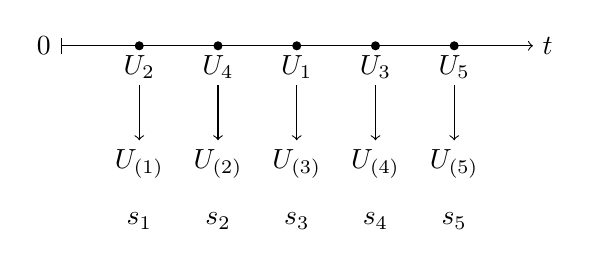
\begin{tikzpicture}
                \draw[|->] (0,0) node[left]{$0$} -- (6, 0) node[right]{$t$};
                \draw[fill] (1, 0) node[below]{$U_2$} circle (0.05);
                \draw[fill] (2, 0) node[below]{$U_4$} circle (0.05);
                \draw[fill] (3, 0) node[below]{$U_1$} circle (0.05);
                \draw[fill] (4, 0) node[below]{$U_3$} circle (0.05);
                \draw[fill] (5, 0) node[below]{$U_5$} circle (0.05);
                \draw[->] (1, -0.5) -- (1, -1.2) node[below]{$U_{(1)}$};
                \draw[->] (2, -0.5) -- (2, -1.2) node[below]{$U_{(2)}$};
                \draw[->] (3, -0.5) -- (3, -1.2) node[below]{$U_{(3)}$};
                \draw[->] (4, -0.5) -- (4, -1.2) node[below]{$U_{(4)}$};
                \draw[->] (5, -0.5) -- (5, -1.2) node[below]{$U_{(5)}$};
                \draw (1, -2) node[below]{$s_{1}$};
                \draw (2, -2) node[below]{$s_{2}$};
                \draw (3, -2) node[below]{$s_{3}$};
                \draw (4, -2) node[below]{$s_{4}$};
                \draw (5, -2) node[below]{$s_{5}$};
            \end{tikzpicture}
        \end{center}
    \end{example}

    Let us see the reason with $N\br{t} = 1$. Suppose we have that $s_1 = s$ and then $W_2 > t - s$ since the second event has not occurs in $\bs{0, t}$. Then we have the pdf,
    \[ f_{s_1 \mid N\br{t} = 1} \br{s} = \f{f_{s_1}\br{s} P\br{W_2 > t - s}}{P\br{N\br{t} = 1}} \ident_{\bs{0, t}}\br{s} \]
    But we know that $W_2$ is distributed exponentially,
    \begin{align*}
    f_{s_1 \mid N\br{t} = 1} \br{s}
    &= \f{ \la e^{-\la s} e^{-\la\br{t - s}}}{\la t e^{-\la t}} \ident_{\bs{0, t}}\br{s} \\
    &= \f{1}{t}\ident_{\bs{0, t}}\br{s}
    \end{align*}
    This is nothing more than the pdf for $\Unif\bs{0, t}$.
    \[ s_1 \mid N\br{t} = 1 \sim \Unif\bs{0, t} \]
    As a result of the order statistics property, we have the following.
    \begin{theorem}
        \[ N\br{s} \mid N\br{t} = n \sim \Bi\br{n, \f{s}{t}} \quad \text{for } s \leq t\]
    \end{theorem}
    The reason being that given $N\br{t} = n$, the order statistics property gives,
    \begin{align*}
        N\br{s}
        &= \# \bc{S_i : S_i \leq s, i = 1, \ldots, n} \\
        &= \# \bc{U_{(i)} : U_{(i)} \leq s, i = 1, \ldots, n} \\
        &= \# \bc{U_{i} : U_{i} \leq s, i = 1, \ldots, n}
    \end{align*}
    The last step validated by the fact that $\bc{U_{(i)}}$ is just a particular permutation of $\bc{U_{i}}$. Therefore $U_i \stackrel{\text{i.i.d}}{\sim} \Unif\bs{0, t}$ because,
    \[ P\br{U_i \leq s} = \f{s}{t} \quad i = 1, \ldots, n \]

    \section{Continuous-time Markov chain}

    The Poisson process is the simplest example of a continuous time process that happens to be a counting process.
    \begin{definition}
        A \term{continuous time stochastic process} $\bc{X\br{t}}_{t \geq 0}$ is called a \term{continuous-time Markov chain} is its state space is at most countable and t satisfies the \term{continuous-time Markov property}.
    \end{definition}
    Recall the continuous-time Markov property (\cref{def:ctmp}),
    \[ P\br{X\br{t_m} = j \mid X\br{t_{m-1}} = i, X\br{t_{m-2}} = i_{m-2}, \ldots, X\br{t_1} = 1} = P\br{X\br{t_{m}} = i \mid X\br{t_{m-1}} = i} \]
    For any $m, t_1 < \cdots < t_m, i_1, \ldots, i_{m-2}, i, j \in S$. As DTMC, $S$ can be considered as finite $\bc{0, \ldots, M}$ or $\bc{1, \ldots, M}$ or countably infinite $\bc{0, 1, \ldots}$, $\bc{0, \pm 1, \pm 2, \ldots} = \Z$. For a CTMC, time is continuous, but the state space is only countable and thus this discrete. Since time is continuous and the state space is discrete, the CTMC must linger or stay at a given state for a finite amount of time and then jump to another state instantaneously.

    \begin{center}
        \begin{tikzpicture}
            \pgfmathsetmacro{\sa}{1};
            \pgfmathsetmacro{\sb}{2};
            \pgfmathsetmacro{\sc}{2.5};
            \pgfmathsetmacro{\sd}{3};
            \pgfmathsetmacro{\se}{3.4};
            \pgfmathsetmacro{\sf}{4};
            \pgfmathsetmacro{\tick}{0.1};
            \pgfmathsetmacro{\jump}{0.4};
            \draw[<->] (0, 3) node[above]{$X\br{t}$} -- (0, 0)node[left]{$0$} -- (5, 0) node[right]{$t$};
            \draw[] (\sa, -\tick) node[below]{$t_1$} -- (\sa, \tick);
            \draw[] (\sb, -\tick) node[below]{$t_2$} -- (\sb, \tick);
            \draw[] (\sc, -\tick) node[below]{$t_3$} -- (\sc, \tick);
            \draw[] (\sd, -\tick) node[below]{$t_4$} -- (\sd, \tick);
            \draw[] (\se, -\tick) node[below]{$t_5$} -- (\se, \tick);
            \draw[] (\sf, -\tick) node[below]{$t_6$} -- (\sf, \tick);
            \draw[thick] (0,\jump) --
            (\sa, 1*\jump) -- (\sa, 3*\jump) --
            (\sb, 3*\jump) -- (\sb, 5*\jump) --
            (\sc, 5*\jump) -- (\sc, 1*\jump) --
            (\sd, 1*\jump) -- (\sd, 4*\jump) --
            (\se, 4*\jump) -- (\se, 2*\jump) --
            (\sf, 2*\jump) -- (\sf, 1*\jump) --
            (5, 1*\jump)
            ;
        \end{tikzpicture}
    \end{center}

    Therefore we need to specify two things:
    \begin{enumerate}
        \item When the jumps happen and how long the process stays in a state?
        \item When it jumps, where does it jump to?
    \end{enumerate}
    To answer the first question, given the process is in state $i$, it will stay in this state for an exponential random time, with parameter denoted $\la_i$. This distribution is fixed by the Markov property. When the process will jump in the future only depends on its current state, not on how long it has been there. Therefore the waiting time must be exponentially distributed. Moreover theMarkov property enforces that the exponential parameter can only depend on state $i$.

    \todo[TC]{Missed a lecture}

    The transition probability when \textit{a jump happens} is defined as,
    \[ q_{ij} \defined P\br{X\br{t} \text{ jumps to } j \mid X\br{t} \text{ jumps from } i} \]
    The transition probability at a jump has the following properties,
    \[ q_{ii} = 0 \quad q_{ij} \geq 0 \quad j\neq i \]
    \[ \sum_{j \in S}q_{ij} = \sum_{j \neq i} q_{ij} = 1 \]
    A CTMC is fully characterized by $\bc{\la_i}_{i \in S}$ and $a = \bc{q_{ij}}_{i,j \in S}$. Moreover the transition probability at a time $t$ is given by,
    \begin{align*}
        P_{ij}\br{t}
        &= P\br{X\br{t} = j \mid X\br{0} = i} \\
        &= P\br{X\br{t+s} = j \mid X\br{s} = i}
    \end{align*}
    And we define the transition matrix at time $t$ to be,
    \[ P\br{t} = \bc{P_{ij}\br{t}}_{i,j \in S} \]
    The continuous C-K equation is simply,
    \[ P\br{t+s} = P\br{t}P\br{s} \]
    \begin{definition}
        The limit
        \[ R \defined \lim_{h \to 0^{+}} \f{P\br{h} - P\br{0}}{h} = \lim_{j \to 0^+} \f{P\br{h} - \ident}{h} \]
        exists, and is called the \term{(infinitesimal) generator matrix} of $\bc{X\br{t}}_{t \geq 0}$.
        \[ R_{ii} = - \la_{i} \quad R_{ij} = \la_i q_{ij} \quad j \neq i \]
        The row sums of $R$ are $0$.
    \end{definition}
    \[ R = \begin{pmatrix}
        -\la_0 & \la_0 q_{01} & \la_0 q_{02} & \cdots \\
        \la_1q_{10} & -\la_{1} & \la_1q_{12} & \cdots \\
        \la_2q_{20} & \la_2q_{21} & -\la_2 & \cdots \\
        \vdots & \vdots & \vdots & \ddots \\
    \end{pmatrix} \]
    The entires of $R$ admit the following intuitive interpretations:
    \begin{itemize}
        \item $-\la_i$: rate/ probability flow going out of state $i$
        \item $\la_i q_{ij}$: rate/ probability flow going from $i$ to $j$
    \end{itemize}
    It is possible to recover $\la_i$ and $q_{ij}$ from $R$. Explicitly,
    \[ \la_i = - R_{ii} \quad q_{ij} = -\f{R_{ij}}{R_{ii}} \quad j \neq i \]
    As we learned previously, the complete set of $\la_i$ and $q_{ij}$ completely characterize the behaviour of the CTMC. Thus, there is a one-to-one relation between $\bc{\la_i}_{i \in S}$ and $\bc{q_{ij}}_{i,j \in S}$. The generator $R$ itself also fully characterizes the CTMC. Therefore,
    \[ \bc{\la_i}_{i \in S} \cup \bc{q_{ij}}_{i,j \in S} \text{ and } \bc{R_{ij}}_{i,j \in S}\]
    are two sets of parameters that can be used to specify a CTMC.

    \begin{example}
        Consider the Poisson process,
        \[ \la_i = \la \quad i = 0, 1, \ldots \]
        \[ Q = \begin{pmatrix}
            0 & 1 & 0 & \cdots \\
            0 & 0 & 1 & \cdots \\
            0 & 0 & 0 & \cdots \\
            \vdots & \vdots & \vdots & \ddots \\
        \end{pmatrix} \]
        From $Q = \bc{q_{ij}}_{i,j \in S}$ and $\bc{\la_i}_{i \in S}$ we can compute $R$:
        \[ R_{ii} = - \la_i = - \la \quad i = 0, 1, \ldots\]
        \[ R_{ij} = \la_i q_{ij} = \begin{cases}
            \la & j = i+1 \\
            0 & j \neq i, i+1 \\
        \end{cases} \]
        \[ R = \begin{pmatrix}
            -\la & \la & 0 & \cdots \\
            0 & -\la & \la & \cdots \\
            0 & 0 & -\la & \cdots \\
            \vdots & \vdots & \vdots & \ddots \\
        \end{pmatrix} \]
        In a Poisson process, the $R_{ij}$ terms are either $-\la, \la$ or $0$.
    \end{example}
    \begin{example}
        Let there be 3 tables in a restaurant. Parties of customers arrive according to a Poisson process with intensity $\la$. Upon arrival, if there are free tables, the party is served and spends an exponential amount of time with average $\f{1}{\mu}$ (parameter $\mu$).\\

        If there are no free tables, the party leaves immediately. Let $X\br{t}$ be the number of occupied tables at time $t$. We know that $S = \bc{0,1,2,3}$ because there are only $3$ tables.\\

        Before we begin, we first need to prove that this process can be modeled as a CTMC. Doing so explicitly is difficult; one would need to prove the Markov Property. Instead we justify that $\bc{X\br{t}}_{t \geq 0}$ by recognizing that all of the interarrival times and service times are independent and exponentially distributed. This assumption generally holds provided that the exponential waiting times are independent. \\

        First find $\la_i$ and $q_{ij}$. First ($i = 0$) $\la_0$ is very easy. The distribution of leaving state $0$ is exponential with parameter corresponding to one party arriving,
        \[ \la_0 = \la \quad \text{leave state $0$ $\iff$ one party arrives}\]
        Moreover,
        \[ q_{01} = 1 \quad \text{zero tables $\implies$ one table} \]
        There is no possible transition from $0$ tables to $i > 1$ tables,
        \[ q_{02} = q_{03} = 0 \]
        For $i = 1$, a new customer can arrive or the current customer can leave,
        \begin{align*}
            1 &\to 2 \quad \text{if next party arrives first} \sim \Ex\br{\la} = T \\
            1 &\to 0 \quad \text{if a service is completed} \sim \Ex\br{\mu} = S
        \end{align*}
        Which one happens first depends on which time is smaller. Recall the property of exponential distribution: $T, S$ are independent,
        \[ T \sim \Ex\br{\la}, S \sim \Ex\br{\mu}, T \indep S \]
        Then,
        \[ P\br{T < S} = \f{\la}{\la + \mu} \quad P\br{S < T} = \f{\mu}{\la + \mu} \]
        Moreover the minimum is exponentially distributed,
        \[ \min\br{T,S} \sim \Ex\br{\la + \mu} \]
        Thus $q_{12} = P\br{T < S} = \la / \br{\la + \mu}$. Additionally,
        \[ q_{10} = 1 - q_{12} = 1 - P\br{T < S} = P\br{S < T} = \f{\mu}{\la + \mu} \]
        We know that $q_{11}$ is zero by definition and $q_{13}$ is zero because that transition is impossible. We also have that $q_{1} = \la + \mu$.\\

        Similarly when two tables are occupied ($i = 2$) there are three possible things that can happen. Let $T \sim \Ex\br{\la}$ be the time until the next arrival just as before. However, there are two possible tables that could leave,
        \[ S_1 \sim \Ex\br{\mu} : \text{service time for table $1$} \]
        \[ S_2 \sim \Ex\br{\mu} : \text{service time for table $2$} \]
        Where $T,S_1,S_2$ are all jointly independent. There are three things that can change the state of the Markov chain.
        \[ \min \br{T, S_1, S_2} \sim \Ex\br{\la + 2 \mu} \]
        We jump from state $2$ to $3$ if there is an arrival before the two services finish.
        \[ P\br{T < S_1, S_2} = \f{\la}{\la+2\mu}\]
        Thus $\la_2 = \la +2\mu$ and,
        \[ q_{23} = \f{\la}{\la+2\mu} \quad q_{21} = \f{2\mu}{\la + 2\mu} \quad q_{20} = q_{22} = 0 \]
        Finally for $i = 3$ no more arrivals can affect the state of the CTMC. Instead there are three possible tables that can complete service. Hence $\la_3 = 3 \mu$ and,
        \[ q_{32} = 1 \quad q_{30} = q_{31} = q_{33} = 0 \]
        Altogether,
        \[ Q = \begin{pmatrix}
            0 & 1 & 0 & 0 \\
            \f{\mu}{\la + \mu} & 0 & \f{\la}{\la + \mu} & 0 \\
            0 & \f{2\mu}{\la + \mu} & 0 & \f{\la}{\la + 2\mu} \\
            0 & 0 & 1 & 0 \\
        \end{pmatrix} \]
        While the intensities are,
        \[ \la_0 = \la \quad \la_1 = \la + \mu \quad \la_2 = \la + 2 \mu \quad \la_3 = 3 \mu \]
        We are also able to calculate the generating matrix $R$.
        \[ R = \begin{pmatrix}
            -\la & \la & 0 & 0 \\
            \mu & -\br{\la + \mu} & \la & 0 \\
            0 & 2 \mu & -\br{\la + 2 \mu} & \la \\
            0 & 0 & 3 \mu & -3\mu \\
        \end{pmatrix} \]
        The entries in $R$ correspond to rates of transition. For example $R_{21}$ is the rate of transition from $2 \to 1$ which equals the total service rate.
    \end{example}
    \begin{remark}
        As can be seen from the previous example, the generating matrix $R$ has a simpler form than $Q$. Actually, $R_{ij}$, $j \neq i$ directly corresponds to the \textit{rate} in which the process moves from state $i$ to $j$. The generating matrix $R$ is also more intuitive. In most cases, the driving force and decaying forces in a CTMC come from different sources. In these cases $R$ is far easier to write down that $Q$. In practice, we often directly model $R$ rather than getting $\bc{\la_i}_{i \in S}$ and $Q = \bc{q_{ij}}_{i,j \in S}$ first.
    \end{remark}
    \begin{example}
        A population model: Each individual gives birth to an offspring with exponential rate $\la$. (i.e. the waiting time until it gets the next offspring $\sim \Ex\br{\la}$). Each individual dies with exponential rate $\mu$. Let $X\br{t}$ be the population at time $t$. When $X\br{t}= i$ there are two possible things that can happen next: either a new birth occurs or a new death occurs. This time until the next (potential) birth is the smallest among the $i$ i.i.d exponential birth times. This means that the ``rate'' from $i$ to $i + 1$ is $i \la$. Similarly, the ``rate'' from $i$ to $i-1$ is $i\mu$.
        \[ R_{i, i+1} = i \la \quad i = 0, 1, \ldots \qquad R_{i, i -1} = i \mu \quad i = 1, 2, \ldots\]
        All of the remaining entires of $R$ will be zero except for the diagonal entires which must fix the row sums of $R$ to be zero.
        \[ R_{ii} = - \br{R_{i, i+1} + R_{i, i-1}} = -i\br{\la + \mu} \]
        Therefore,
        \[ R = \begin{pmatrix}
            0 & 0 & 0 & 0 & \cdots \\
            \mu & -\br{\la+\mu} & \la & 0 & \cdots \\
            0 & 2\mu & -2\br{\la+\mu} & 2\la & \cdots \\
            0 & 0 & 3 \mu & -3\br{\la+\mu} & \cdots \\
            \vdots & \vdots & \vdots & \vdots & \ddots \\
        \end{pmatrix} \]
        Note that the first row is all zeros. Intuitively this corresponds to the fact that state $0$ is an absorbing state. If the population is empty, then no changes can occur to the CTMC. At this point we have completely modeled the CTMC. Albeit if we do need to know $\bc{\la_i}_{i \in S}$ and $Q$ we have that,
        \[ \la_i = - R_{ii} = i \br{\la + \mu} \]
        And,
        \[ q_{i, i+1} = \f{R_{i, i+1}}{- R_{ii}} = \f{i \la}{ i  \br{\la + \mu}} = \f{\la}{\la + \mu} \quad i \geq 1 \]
        Similarly,
        \[ q_{i, i-1} = \f{\mu}{\la + \mu} \quad i \geq 1 \]
        The boundary term $q_{01} = 1$ is arbitrary since $\la_0 = 0$ anyway.
        \[ Q = \begin{pmatrix}
            0 & 1 & 0 & 0 & \cdots \\
            \f{\mu}{\la + \mu} & 0 & \f{\la}{\la + \mu} & 0 & \cdots \\
            0 & \f{\mu}{\la + \mu} & 0 & \f{\la}{\la + \mu} & \cdots \\
            0 & 0 & \f{\mu}{\la + \mu} & 0 & \cdots \\
            \vdots & \vdots & \vdots & \vdots & \ddots \\
        \end{pmatrix} \]
    \end{example}
    So far our population model only incorporated births and deaths of individuals. We can further add immigration to the system. Individuals are added to the population according to a Poisson process with intensity $\al$. It is important to note that this augmentation will not change the ``rate'' of transitions from $i$ to $i-1$. Intuitively, the immigration rate does not affect the death rate of the population. Instead, the immigration model changes the rate of transition from $i$ to $i + 1$. \\

    If we look at the time until the next increase in population, it now the minimum of two random variables (time until next birth, time until next immigration) following,
    \[ \Ex\br{i \la} \text{ and } \Ex\br{\al} \]
    Where $\Ex\br{i \la}$ is associated to the birth rate. Each of the $i$ individuals can give birth with intensity $\la$. The immigration interarrival times are $\Ex\br{\al}$ and are independent of $i$. Therefore the rate from $i$ to $i+1$ is now $i \la + \al$,
    \[ R = \begin{pmatrix}
        -\al & \al & 0 & 0 & \cdots \\
        \mu & -\br{\la+\mu}-\al & \la + \al & 0 & \cdots \\
        0 & 2\mu & -2\br{\la+\mu}-\al & 2\la + \al & \cdots \\
        0 & 0 & 3 \mu & -3\br{\la+\mu}-\al & \cdots \\
        \vdots & \vdots & \vdots & \vdots & \ddots \\
    \end{pmatrix} \]
    Entry-wise,
    \[ R_{i, i-1} = i \mu \quad i = 1,2,\ldots \]
    \[ R_{i, i+1} = i \la + \al \quad i = 0,2,\ldots \]
    $\bc{\la_i}_{i \in S}$ and $Q$ will change accordingly.

    \subsection{Classification of States}

    Just as we classified states in a DTMC, we attempt to classify states in a CTMC in an analogous manner. We will do this by examining properties of $Q$. Recall that,
    \[ q_{ij} = P\br{X\br{t} \text{ jumps to $j$ } \mid X\br{t} \text{ jumps from $i$ } } \]
    Where $q_{ij} \geq 0$ and $\sum_{j\in S} q_{ij} = 1$. If we collect all of the entries $\bc{q_{ij}}_{i,j\in S}$ into $Q$, $Q$ becomes a legitimate transition matrix of a DTMC. \\

    To see how the CTMC is related to the corresponding DTMC, consider the following arbitrary depiction of a CTMC $\bc{X\br{t}}_{t \geq 0}$,
    \begin{center}
        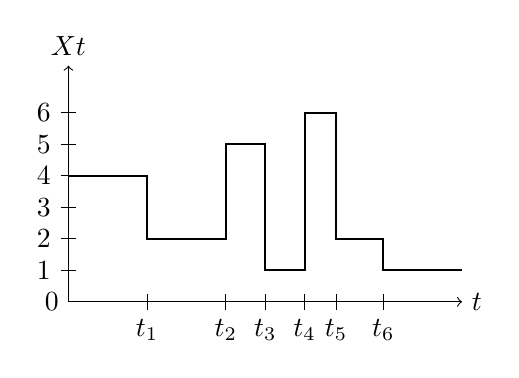
\begin{tikzpicture}
            \pgfmathsetmacro{\sa}{1};
            \pgfmathsetmacro{\sb}{2};
            \pgfmathsetmacro{\sc}{2.5};
            \pgfmathsetmacro{\sd}{3};
            \pgfmathsetmacro{\se}{3.4};
            \pgfmathsetmacro{\sf}{4};
            \pgfmathsetmacro{\tick}{0.1};
            \pgfmathsetmacro{\jump}{0.4};
            \draw[<->] (0, 3) node[above]{$X\br{t}$} -- (0, 0)node[left]{$0$} -- (5, 0) node[right]{$t$};
            \draw[] (\sa, -\tick) node[below]{$t_1$} -- (\sa, \tick);
            \draw[] (\sb, -\tick) node[below]{$t_2$} -- (\sb, \tick);
            \draw[] (\sc, -\tick) node[below]{$t_3$} -- (\sc, \tick);
            \draw[] (\sd, -\tick) node[below]{$t_4$} -- (\sd, \tick);
            \draw[] (\se, -\tick) node[below]{$t_5$} -- (\se, \tick);
            \draw[] (\sf, -\tick) node[below]{$t_6$} -- (\sf, \tick);
            \draw[] (-\tick, 1*\jump) node[left]{$1$} -- (\tick, 1*\jump);
            \draw[] (-\tick, 2*\jump) node[left]{$2$} -- (\tick, 2*\jump);
            \draw[] (-\tick, 3*\jump) node[left]{$3$} -- (\tick, 3*\jump);
            \draw[] (-\tick, 4*\jump) node[left]{$4$} -- (\tick, 4*\jump);
            \draw[] (-\tick, 5*\jump) node[left]{$5$} -- (\tick, 5*\jump);
            \draw[] (-\tick, 6*\jump) node[left]{$6$} -- (\tick, 6*\jump);
            \draw[thick] (0,4*\jump) --
            (\sa, 4*\jump) -- (\sa, 2*\jump) --
            (\sb, 2*\jump) -- (\sb, 5*\jump) --
            (\sc, 5*\jump) -- (\sc, 1*\jump) --
            (\sd, 1*\jump) -- (\sd, 6*\jump) --
            (\se, 6*\jump) -- (\se, 2*\jump) --
            (\sf, 2*\jump) -- (\sf, 1*\jump) --
            (5, 1*\jump)
            ;
        \end{tikzpicture}
    \end{center}
    We can construct a DTMC by ignoring the interarrival times $t_{k+1} - t_{k}$ and only record the states at each interarrival time. The $1$-step transition probability matrix is given by $Q$. It contains all of the state changes but forgets the temporal information. This DTMC is called the \term{discrete skeleton} or \term{embedded DTMC} of the CTMC.\\

    Since accessibility is the notion that $i$ can go to $j$ in an arbitrary time, we naturally define accessibility in a CTMC between $i$ and $j$ if they are accessible in the discrete skeleton. Moreover communication, irreducibility are derivative of the notion of accessibility and thus we extend the notion as well. \\

    Additionally, the notion of recurrence/transience are also independent of the notion of time and thus are the same in the CTMC as they are in the discrete skeleton. \\

    Since accessibility, communication, irreducibility, recurrence/transience are only related to the change of states, not about time, these properties will be the same for a CTMC and its discrete skeleton. For a CTMC $\bc{X\br{t}}_{t \geq 0}$ we call ``state $j$ accessible from state $i$'' or ``$i$ and $j$ communicate'', ``the process is irreducible'', ``$i$ is recurrent/transient'' if and only if this is the case for its discrete skeleton. \\

    Note that since positive/null recurrence do involve the (expected) amount of time, we can indeed have different results for a CTMC and its discrete skeleton. In particular we need to define positive/null recurrence for a CTMC.
    \begin{definition}
        Let $R_{ii}$ be the amount of (continuous) time until the MC revisits state $i$ given $X\br{0}= i$. A recurrent state $i$ is called positive recurrent if $\Exp\br{R_{ii}}< \inf$.
        \[\text{$i$ is positive recurrent: } \quad \Exp\br{R_{ii}}< \inf\]
        It is called null recurrent if $\Exp\br{R_{ii}} = \inf$.
        \[\text{$i$ is null recurrent: } \quad \Exp\br{R_{ii}} = \inf\]
    \end{definition}
    \begin{center}
        \begin{tikzpicture}
            \pgfmathsetmacro{\sa}{1};
            \pgfmathsetmacro{\sb}{2};
            \pgfmathsetmacro{\sc}{2.5};
            \pgfmathsetmacro{\sd}{3};
            \pgfmathsetmacro{\se}{3.4};
            \pgfmathsetmacro{\sf}{4};
            \pgfmathsetmacro{\tick}{0.1};
            \pgfmathsetmacro{\jump}{0.4};
            \draw[<->] (0, 3) node[above]{$X\br{t}$} -- (0, 0)node[left]{$0$} -- (5, 0) node[right]{$t$};
            \draw[] (\sa, -\tick) -- (\sa, \tick);
            \draw[] (\sb, -\tick) -- (\sb, \tick);
            \draw[] (\sc, -\tick) -- (\sc, \tick);
            \draw[] (\sd, -\tick) -- (\sd, \tick);
            \draw[] (\se, -\tick) -- (\se, \tick);
            \draw[] (\sf, -\tick) node[below]{$R_{ii}$} -- (\sf, \tick);
            \draw[] (-\tick,4*\jump) node[left]{$i$} -- (\tick, 4*\jump);
            \draw[thick] (0,4*\jump) -- (\sa, 4*\jump);
            \draw[thick, dashed] (\sa, 4*\jump) -- (\sa, 2*\jump);
            \draw[thick, dashed] (\sa, 2*\jump) -- (\sb, 2*\jump);
            \draw[thick, dashed] (\sb, 2*\jump) -- (\sb, 5*\jump);
            \draw[thick, dashed] (\sb, 5*\jump) -- (\sc, 5*\jump);
            \draw[thick, dashed] (\sc, 5*\jump) -- (\sc, 1*\jump);
            \draw[thick, dashed] (\sc, 1*\jump) -- (\sd, 1*\jump);
            \draw[thick, dashed] (\sd, 1*\jump) -- (\sd, 6*\jump);
            \draw[thick, dashed] (\sd, 6*\jump) -- (\se, 6*\jump);
            \draw[thick, dashed] (\se, 6*\jump) -- (\se, 2*\jump);
            \draw[thick, dashed] (\se, 2*\jump) -- (\sf, 2*\jump);
            \draw[thick, dashed] (\sf, 2*\jump) -- (\sf, 4*\jump);
            \draw[thick] (\sf, 4*\jump) -- (5, 4*\jump) -- (5, 4*\jump);
        \end{tikzpicture}
    \end{center}
    As in the discrete case positive recurrence, null recurrence and transience are class properties. However positive/null recurrences can be different for a DTMC and its discrete skelton, but they are still class properties.
    \subsection{Stationary Distribution}
    \begin{definition}
        A distribution $\pi = \br{\pi_0, \pi_1, \ldots}$ is called a \term{stationary distribution} of a CTMC $\bc{\la\br{t}}_{t \geq 0}$ with generator $R$, iff it satisfies:
        \[ \pi \cdot R = 0 \quad \sum_{i} \pi_i = \pi \cdot \ve 1 = 1 \]
        Notice that the first condition differs from the discrete case where $\pi \cdot P = \pi$.
    \end{definition}
    Why do we call $\pi$ stationary distributions? To see that $\pi$ is fixed, assume that the process starts by initial distribution $\al^{(0)} = \pi$:
    \[ P\br{X\br{0} =  i} = \pi_i \]
    The distribution of this process at time $t$ is given by,
    \[ \al^{(t)} = \al^{(0)} \cdot P\br{t} = \pi \cdot P \br{t} \]
    This is obtained by looking at $\al_{j}^{(t)}$:
    \begin{align*}
    \al_j^{(t)}
    &= P\br{X\br{t} = j} \\
    &= \sum_{i\in S}P\br{X\br{t} = j \mid X\br{0} = i}P\br{X\br{0} = i} \\
    &= \sum_{i\in S}P_{ij}\br{t}\al_{i}^{(0)} \\
    &= \br{\al^{(0)} \cdot P\br{t}}_{j}
    \end{align*}
    To show that $\al^{(t)}$ is constant in time, examine,
    \begin{align*}
        \der{\al^{(t)}}{t}
        &= \der{}{t} \br{\al^{(0)} \cdot P\br{t}}\\
        &= \der{}{t} \br{\pi \cdot P\br{t}}\\
        &= \pi \cdot \der{}{t} P\br{t} \\
        &= \pi \cdot \br{\lim_{h \to 0^{+}} \f{P\br{t + h} - P\br{t}}{h}} \\
        &= \pi \cdot \br{\lim_{h \to 0^{+}} \f{P\br{t}\cdot P\br{h} - P\br{t}}{h}} \quad \text{C-K equation} \\
        &= \pi \cdot \br{\lim_{h \to 0^{+}} \f{P\br{h} - \ident}{h}} \cdot P\br{t} \\
        &= \pi \cdot R \cdot P\br{t} \\
        &= \ve 0\cdot P\br{t} \\
        &= \ve 0
    \end{align*}
    This means that $\al^{(t)}$ does not change with time. It is a constant vector. In other words, the distribution of $X\br{t}$ will not change over time if the MC starts from the stationary distribution.
    \begin{theorem}
        If a CTMC starts from a stationary distribution $\pi$, then its distribution will never change.
    \end{theorem}
    \begin{theorem}
        \label{thm:bltctmc}
        \term{Basic Limit Theorem for CTMC}: Let $\bc{X\br{t}}_{t \geq 0}$ be an irreducible, recurrent CTMC. Then $\pi_{j}$ exists and also:
        \[ \lim_{t \to \inf} P_{ij}\br{t} = \pi_{j} = \f{\Exp\br{T_j}}{\Exp\br{R_{jj}}} = \f{1 / \la_{j}}{\Exp\br{R_{jj}}} \quad \forall i, j \in S \]
        In addition, the MC is positive recurrent if and only if a unique stationary distribution exists. In this case, the unique stationary distribution is the $\pi = \br{\pi_{0}, \pi_{1}, \ldots}$ where $\pi_j$ is mentioned above.
    \end{theorem}
    Note that the last equality in \cref{thm:bltctmc} holds because $T_{j}$ is distributed exponentially will expectation $1 / \la_j$. Most of the terms and relations that hold for \cref{thm:bltctmc} are analogous to the discrete case.
    \begin{remark}
        The long-run fraction of time spent in state $j$ is given by $\Exp\br{T_j}/ \Exp\br{R_{jj}}$. The idea being that $R_{jj}$ represents the amount of time until the first return to state $j$ given that we started in state $j$ at time $0$.
        \begin{center}
            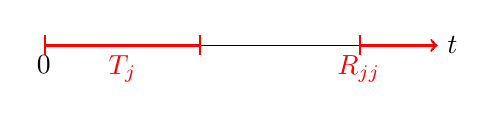
\begin{tikzpicture}
                \draw[|->] (0,0) node[below]{$0$} -- (5, 0) node[right]{$t$};
                \draw[red,thick,|-|] (0,0) -- node[below]{$T_j$} (2, 0);
                \draw[|->, red,thick] (4,0) node[below]{$R_{jj}$} -- (5, 0);
            \end{tikzpicture}
        \end{center}
        For each interval of length $R_{jj}$, $T_{j}$ is the portion of time spent in state $j$.
    \end{remark}

    \subsection{Birth and Death Process}
    \begin{definition}
        A \term{birth and death process} is a CTMC such that,
        \[ S = \bc{0, 1,\ldots,m} \text{ or } S = \bc{0, 1,\ldots} \]
        and that,
        \[ q_{i, i - 1} + q_{i, i + 1} = 1 \quad \forall i \in S\]
        This later condition is identical to enforcing that,
        \[ q_{ij} = 0 \quad \forall j \in S, \br{j \neq i \pm 1} \]
        The process can only change to the neighboring states.
    \end{definition}
    For a birth and death process we use a new set of parameters. Denote:
    \[ \la_i = R_{i, i + 1} \quad i = 0, 1, 2, \ldots \]
    \[ \mu_i = R_{i, i - 1} \quad \mu = 1, 2, \ldots \]
    \[ R = \begin{pmatrix}
        - \la_0 & \la_0 & 0 & 0 & 0 & \ldots \\
        \mu_1 & -\br{\la_1 + \mu_1} & \la_1 & 0 & 0 & \ldots \\
        0 & \mu_2 & -\br{\la_2 + \mu_2} & \la_2 & 0 & \ldots \\
        0 & 0 & \mu_3 & -\br{\la_3 + \mu_3} & \la_4 & \ldots \\
        0 & 0 & 0 & \mu_4 & -\br{\la_4 + \mu_4} & \ldots \\
        \vdots & \vdots & \vdots & \vdots & \vdots & \ddots \\
    \end{pmatrix} \]
    Where $R_{00} = - \la_0$ always and $R_{ii} = -\br{\la_i + \mu_i}$ for all entries where $i = 1,2,\ldots$. We have the following interpretation of the entires,
    \[ \text{$\la_{i}$'s are called \term{birth rates}} \]
    \[ \text{$\mu_{i}$'s are called \term{death rates}} \]
    Most of the processes we have consider thus far are actually birth and death processes.
    \begin{example}
        Consider our previous example of the restaurant with three tables.
        \[ R = \begin{pmatrix}
            - \la & \la & 0 & 0 \\
            1\mu & -\br{\la + \mu} & \la & 0 \\
            0 & 2\mu & -\br{\la + 2\mu} & \la \\
            0 & 0 & 3\mu & -3\mu \\
        \end{pmatrix} \]
        This is a birth and death process with the following rates.
        \[ \text{Birth rate:} \quad \la_i = \la \quad i = 0, 1, 2\ldots  \]
        \[ \text{Death rate:} \quad \mu_i = i\mu \quad i = 1, 2\ldots  \]
    This birth and death system is actually part of a larger family of processes. In general consider a \term{$m/m/s$ queuing system}. The first $m$ indicates that there is an exponential interarrival time $\stackrel{\text{i.i.d}}{\sim} \Ex\br{\la}$. The second $m$ indicates that there is an exponential service time $\stackrel{\text{i.i.d}}{\sim} \Ex\br{\mu}$. The final $s$ indicates that there are $s$ servers. There are two limiting/degenerate cases for $s$. In the case that $s$ equals $1$, then there is only one server and the queue is trivial. Alternatively, if $s = \inf$ then all customers that arrive are served. In general we let $X\br{t}$ be the number of customers in the system at time $t$. A queuing system is a birth and death system because a birth rate corresponds to the arrival times of customers.
    \[ \la_i = \la \quad i = 0, 1, \ldots\]
    Moreover the death rate corresponds to the completion of a service. When there are $X\br{t} = i$ customers in the system there are two cases,
    \begin{enumerate}
        \item If $i \leq s$ then $i$ servers are busy each with $\sim \Ex\br{\mu}$. The total death rate,
        \[ \mu_i = i \mu \]
        \item If $i \geq s$ then all $s$ servers will be busy and we will have a queue. The total death rate is capped,
        \[ \mu_i = s \mu \]
    \end{enumerate}
    Thus for an $m/m/s$ queue we have,
    \begin{align*}
    \la_i &= \la \qquad i = 0, 1,\ldots  \\
    \mu_i &= \begin{cases}
        i \mu & i\leq s \\
        s \mu & i > s
    \end{cases}
    \end{align*}
    \end{example}
    \begin{example}
        Consider an actual population model where the birth and death process is literal.
        \[ R = \begin{pmatrix}
            - \al & \al & 0 & 0 & \ldots \\
            \mu & -\br{\la +\mu + \al} & \la+ \al & 0 & \ldots \\
            0 & 2\mu & -\br{2{\la +\mu} + \al} & 2\la +\al & \ldots \\
            \vdots & \vdots & \vdots & \vdots  & \ddots \\
        \end{pmatrix} \]
        The birth rate is at state $i$ is $i \la + \mu$ where $i = 0, 1,\ldots$. Note that this is not the \textit{biological} birth rate but the total rate by which the process goes from $i$ to $i + 1$. The death rate is simply $\mu_i = i \mu$ for $i = 1,2,\ldots$.
    \end{example}
    As we see, there are two main types of birth and deaths processes: queuing system and population model.
    A queuing system and the population model are both birth and death processes by have a few qualitative differences.
    The key difference between them is that the birth rate in the queuing system is typically a constant (the number of customers arriving doesn't depend on the number of existing customers; it does not depend on state $i$) while the birth rate in the population model increases was $i$ increases. \\

    Both these models are worth studying for practical reasons but there is also an analytic advantage; in these simple systems, the form of the generating matrix $R$ is not complicated. As it turns out, it is possible to analytically calculate the stationary distribution.\\

    To find the stationary distribution of a birth and death process we need to find $\pi$ such that,
    \[ \pi \cdot R = 0 \qquad \pi \cdot \ve 1 = 1 \quad \pi = \br{\pi_0, \pi_1, \ldots} \]
    Where we recall that $R$ has the generic form,
    \[ R = \begin{pmatrix}
        - \la_0 & \la_0 & 0 & 0 & 0 & \ldots \\
        \mu_1 & -\br{\la_1 + \mu_1} & \la_1 & 0 & 0 & \ldots \\
        0 & \mu_2 & -\br{\la_2 + \mu_2} & \la_2 & 0 & \ldots \\
        0 & 0 & \mu_3 & -\br{\la_3 + \mu_3} & \la_4 & \ldots \\
        0 & 0 & 0 & \mu_4 & -\br{\la_4 + \mu_4} & \ldots \\
        \vdots & \vdots & \vdots & \vdots & \vdots & \ddots \\
    \end{pmatrix} \]
    The first row gives us,
    \[ -\la_0 \pi_0 + \mu_1 \pi_1 = 0 \implies \pi_1 = \f{\la_0}{\mu_1} \pi_0 \]
    The second row gives us a more involved result,
    \[ -\la_0 \pi_0 - \br{\mu_1 + \la_1} \pi_1 + \mu_2 \pi_2 = 0 \]
    If we add this to the first equation we get,
    \[ -\la_1 \pi_1 + \mu_2 \pi_2 = 0 \implies \pi_2 = \f{\la_1}{\mu_2} \pi_1 \]
    But we already know that $\pi_1$ can be written in terms of $\pi_0$,
    \[ \pi_2 = \f{\la_1 \la_0}{\mu_2 \mu_1} \pi_0 \]
    If we continue this process, we arrive at the general term of,
    \[ \pi_n = \f{\la_0 \cdots \la_{n-1}}{\mu_1 \cdots \mu_n} \pi_0 = \prod_{j=1}^{n}\f{\la_{j-1}}{\mu_j} \pi_0 \]
    These equations fix all entries of $\pi$ up to a normalization. If we sum over all entries (taking the special case of $\pi_i$ into account),
    \[ 1 = \sum_{n=0}^{\inf} \pi_n = \br{1+ \sum_{n=0}^{\inf} \prod_{j=1}^{n}\f{\la_{j-1}}{\mu_j}} \pi_0 \]
    Therefore we have $\pi_0$,
    \[ \pi_0 = \br{1+ \sum_{n=0}^{\inf} \prod_{j=1}^{n}\f{\la_{j-1}}{\mu_j}}^{-1} \]
    While the remaining entries are,
    \[ \pi_n = \prod_{j=1}^{n}\f{\la_{j-1}}{\mu_j}\br{1+ \sum_{n=0}^{\inf} \prod_{j=1}^{n}\f{\la_{j-1}}{\mu_j}}^{-1} \]
    Of course, the uniqueness of a stationary distribution is contingent on the fact that the CTMC is positive recurrent. It is not true for all birth and death processes so it must be that positive recurrence can be determined by the convergence of $\pi_0$. Therefore we have that a stationary distribution $\pi$ exists (and thus MC is positive recurrent) and is normalizable if,
    \[ \sum_{n=0}^{\inf} \prod_{j=1}^{n}\f{\la_{j-1}}{\mu_j} < \inf \]
    One would fear that these expressions are quite complicated and would be difficult to work out explicitly. However consider the case of a $m/m/s$ queue. Recall that $\la_i = \la$ and $\mu_i = i \mu$ if $i \leq s$ and $\mu_i = s \mu$ if $i \geq s$. Therefore,
    \[ \sum_{n=0}^{\inf} \prod_{j=1}^{n}\f{\la_{j-1}}{\mu_j} = \f{\la}{\mu} + \f{\la}{\mu} \f{\la}{2\mu} + \cdots + \f{\la}{\mu}\f{\la}{2\mu}\cdots \f{\la}{s\mu} + \f{\la}{\mu}\f{\la}{2\mu}\cdots \br{\f{\la}{s\mu}}^2 +\cdots \]
    The first $s$ terms correspond to a finite sum and is thus finite. The remaining terms are,
    \[ \sum_{n=0}^{\inf} \prod_{j=s}^{n}\f{\la_{j-1}}{\mu_j} = \f{\la}{\mu}\f{\la}{2\mu}\cdots \br{\f{\la}{s\mu}}^2 + \f{\la}{\mu}\f{\la}{2\mu}\cdots \br{\f{\la}{s\mu}}^3 + \cdots \]
    Which is a geometric series we parameter $\f{\la}{s\mu}$. Therefore the sum is finite if and only if $\la < s \mu$. The process is positive recurrent if and only if,
    \[ \la < s \mu \]


\end{document}